% VUT FIT MITAI
% MSZ 2021/2022
% Author: Vladimir Dusek
% Login: xdusek27

%%%%%%%%%%%%%%%%%%%%%%%%%%%%%%%%%%%%%%%%%%%%%%%%%%%%%%%%%%%%%%%%%%%%%%%%%%%%%%%%

\documentclass{fitthesis}

\usepackage[english,czech]{babel}
\usepackage[utf8]{inputenc}
\usepackage[T1]{fontenc}
\usepackage{geometry}
\usepackage{listings}
\usepackage{amsmath}
\usepackage{amssymb}
\usepackage[justification=centering]{caption}
\usepackage{subcaption}
\usepackage{graphicx}
\usepackage[ruled,vlined,linesnumbered]{algorithm2e}
\usepackage{float}
\usepackage{xcolor}
\usepackage{csquotes}
\usepackage[bottom]{footmisc}
\usepackage[nottoc,numbib]{tocbibind}
\usepackage{hhline}
\usepackage{pdfpages}
\usepackage{mathtools}

\newtheorem{theorem}{Theorem}

\makeatletter
\renewcommand*\env@matrix[1][*\c@MaxMatrixCols c]{%
    \hskip -\arraycolsep
    \let\@ifnextchar\new@ifnextchar
    \array{#1}}
\makeatother

\MakeOuterQuote{"}

\PassOptionsToPackage{hyphens}{url}\usepackage[hidelinks,unicode]{hyperref}

% Page dimensions
\geometry
{
    top = 3cm,
    bottom = 3cm,
    left = 3cm,
    right = 3cm
    % text = {17cm, 24cm}
}

% Path for figures
\graphicspath{{figures/}}

% Listing styles colors
\colorlet{punct}{red!60!black}
\definecolor{background}{HTML}{EEEEEE}
\definecolor{delim}{RGB}{20,105,176}
\colorlet{numb}{magenta!60!black}

% Listing style for JSON
\lstdefinelanguage{json}{
    basicstyle=\small\ttfamily,
    numbers=none,
    showstringspaces=false,
    breaklines=true,
    frame=none,
    backgroundcolor=\color{background},
    morecomment=[l]{//}, % l is for line comment
    literate=%
        % {0}{{{\color{numb}0}}}{1}
        % {1}{{{\color{numb}1}}}{1}
        % {2}{{{\color{numb}2}}}{1}
        % {3}{{{\color{numb}3}}}{1}
        % {4}{{{\color{numb}4}}}{1}
        % {5}{{{\color{numb}5}}}{1}
        % {6}{{{\color{numb}6}}}{1}
        % {7}{{{\color{numb}7}}}{1}
        % {8}{{{\color{numb}8}}}{1}
        % {9}{{{\color{numb}9}}}{1}
        {:}{{{\color{punct}{:}}}}{1}
        {,}{{{\color{punct}{,}}}}{1}
        {\{}{{{\color{delim}{\{}}}}{1}
        {\}}{{{\color{delim}{\}}}}}{1}
        {[}{{{\color{delim}{[}}}}{1}
        {]}{{{\color{delim}{]}}}}{1}
        {á}{{\'a}}1
        {í}{{\'i}}1
        {é}{{\'e}}1
        {ý}{{\'y}}1
        {ú}{{\'u}}1
        {ó}{{\'o}}1
        {ě}{{\v{e}}}1
        {š}{{\v{s}}}1
        {č}{{\v{c}}}1
        {ř}{{\v{r}}}1
        {ž}{{\v{z}}}1
        {ď}{{\v{d}}}1
        {ť}{{\v{t}}}1
        {ň}{{\v{n}}}1
        {ů}{{\r{u}}}1
        {Á}{{\'A}}1
        {Í}{{\'I}}1
        {É}{{\'E}}1
        {Ý}{{\'Y}}1
        {Ú}{{\'U}}1
        {Ó}{{\'O}}1
        {Ě}{{\v{E}}}1
        {Š}{{\v{S}}}1
        {Č}{{\v{C}}}1
        {Ř}{{\v{R}}}1
        {Ž}{{\v{Z}}}1
        {Ď}{{\v{D}}}1
        {Ť}{{\v{T}}}1
        {Ň}{{\v{N}}}1
        {Ů}{{\r{U}}}1
}

% Listing style for Bash
\lstdefinelanguage{bash}{
    basicstyle=\small\ttfamily,
    numbers=none,
    showstringspaces=false,
    breaklines=true,
    frame=none,
    backgroundcolor=\color{background},
    showlines=true
}

% Listing style for Python
\lstdefinelanguage{python}{
    basicstyle=\small\ttfamily,
    numbers=left,
    showstringspaces=false,
    keywordstyle=\color{numb},
    % list of keywords
    morekeywords={
        import,
        if,
        while,
        for,
        then,
        else,
        def,
        True,
        False,
        self,
        return,
        in
    },
    sensitive=false, % keywords are not case-sensitive
    morestring=[b]" % defines that strings are enclosed in double quotes
    breaklines=true,
    frame=none,
    backgroundcolor=\color{background},
    morecomment=[l]{\#}, % l is for line comment
    literate=%
        {:}{{{\color{delim}{:}}}}{1}
        {,}{{{\color{delim}{,}}}}{1}
        {(}{{{\color{delim}{(}}}}{1}
        {)}{{{\color{delim}{)}}}}{1}
        {\{}{{{\color{delim}{\{}}}}{1}
        {\}}{{{\color{delim}{\}}}}}{1}
}

% Listing style for YAML
\lstdefinelanguage{yaml}{
    keywords={true,false,null,y,n},
    keywordstyle=\color{darkgray}\bfseries,
    basicstyle=\YAMLkeystyle,                                 % assuming a key comes first
    sensitive=false,
    comment=[l]{\#},
    morecomment=[s]{/*}{*/},
    commentstyle=\color{purple}\ttfamily,
    stringstyle=\YAMLvaluestyle\ttfamily,
    moredelim=[l][\color{orange}]{\&},
    moredelim=[l][\color{magenta}]{*},
    moredelim=**[il][\YAMLcolonstyle{:}\YAMLvaluestyle]{:},   % switch to value style at :
    morestring=[b]',
    morestring=[b]",
    literate =    {---}{{\ProcessThreeDashes}}3
                  {>}{{\textcolor{red}\textgreater}}1
                  {|}{{\textcolor{red}\textbar}}1
                  {\ -\ }{{\mdseries\ -\ }}3,
}

%%%%%%%%%%%%%%%%%%%%%%%%%%%%%%%%%%%%%%%%%%%%%%%%%%%%%%%%%%%%%%%%%%%%%%%%%%%%%%%%

\begin{document}

\begin{titlepage}
    \begin{center}

        % {\Huge\textsc{Vysoké učení technické v~Brně}} \\
        % \bigskip
        % {\huge\textsc{Fakulta informačních technologií}} \\

        \begin{figure}[htb]
            \centering
            
\includegraphics[width=0.85\hsize]{fitlogo.pdf}
        \end{figure}

        \vspace{\stretch{0.382}}

        {\Huge Vypracované otázky k MSZ pro rok 2022} \\
        \bigskip
        \bigskip
        {\LARGE Specializace NNET}

        \vspace{\stretch{0.618}}
    \end{center}

    {\Large \today \hfill Vladimír Dušek, xdusek27}

\end{titlepage}

% \begin{center}
%     {\Huge Game Theory (THE)} \\ [1.25em]
%     {\huge Brno University of Technology} \\ [1.25em]
%     {\huge Strategie sobeckého těžení v~Bitcoinu} \\ [1.6em]
%     {\Large \textit{Dušek Vladimír - xdusek27@stud.fit.vutbr.cz}} \\ [0.7em]
%     {\Large \textit{\today}}
%  \end{center}

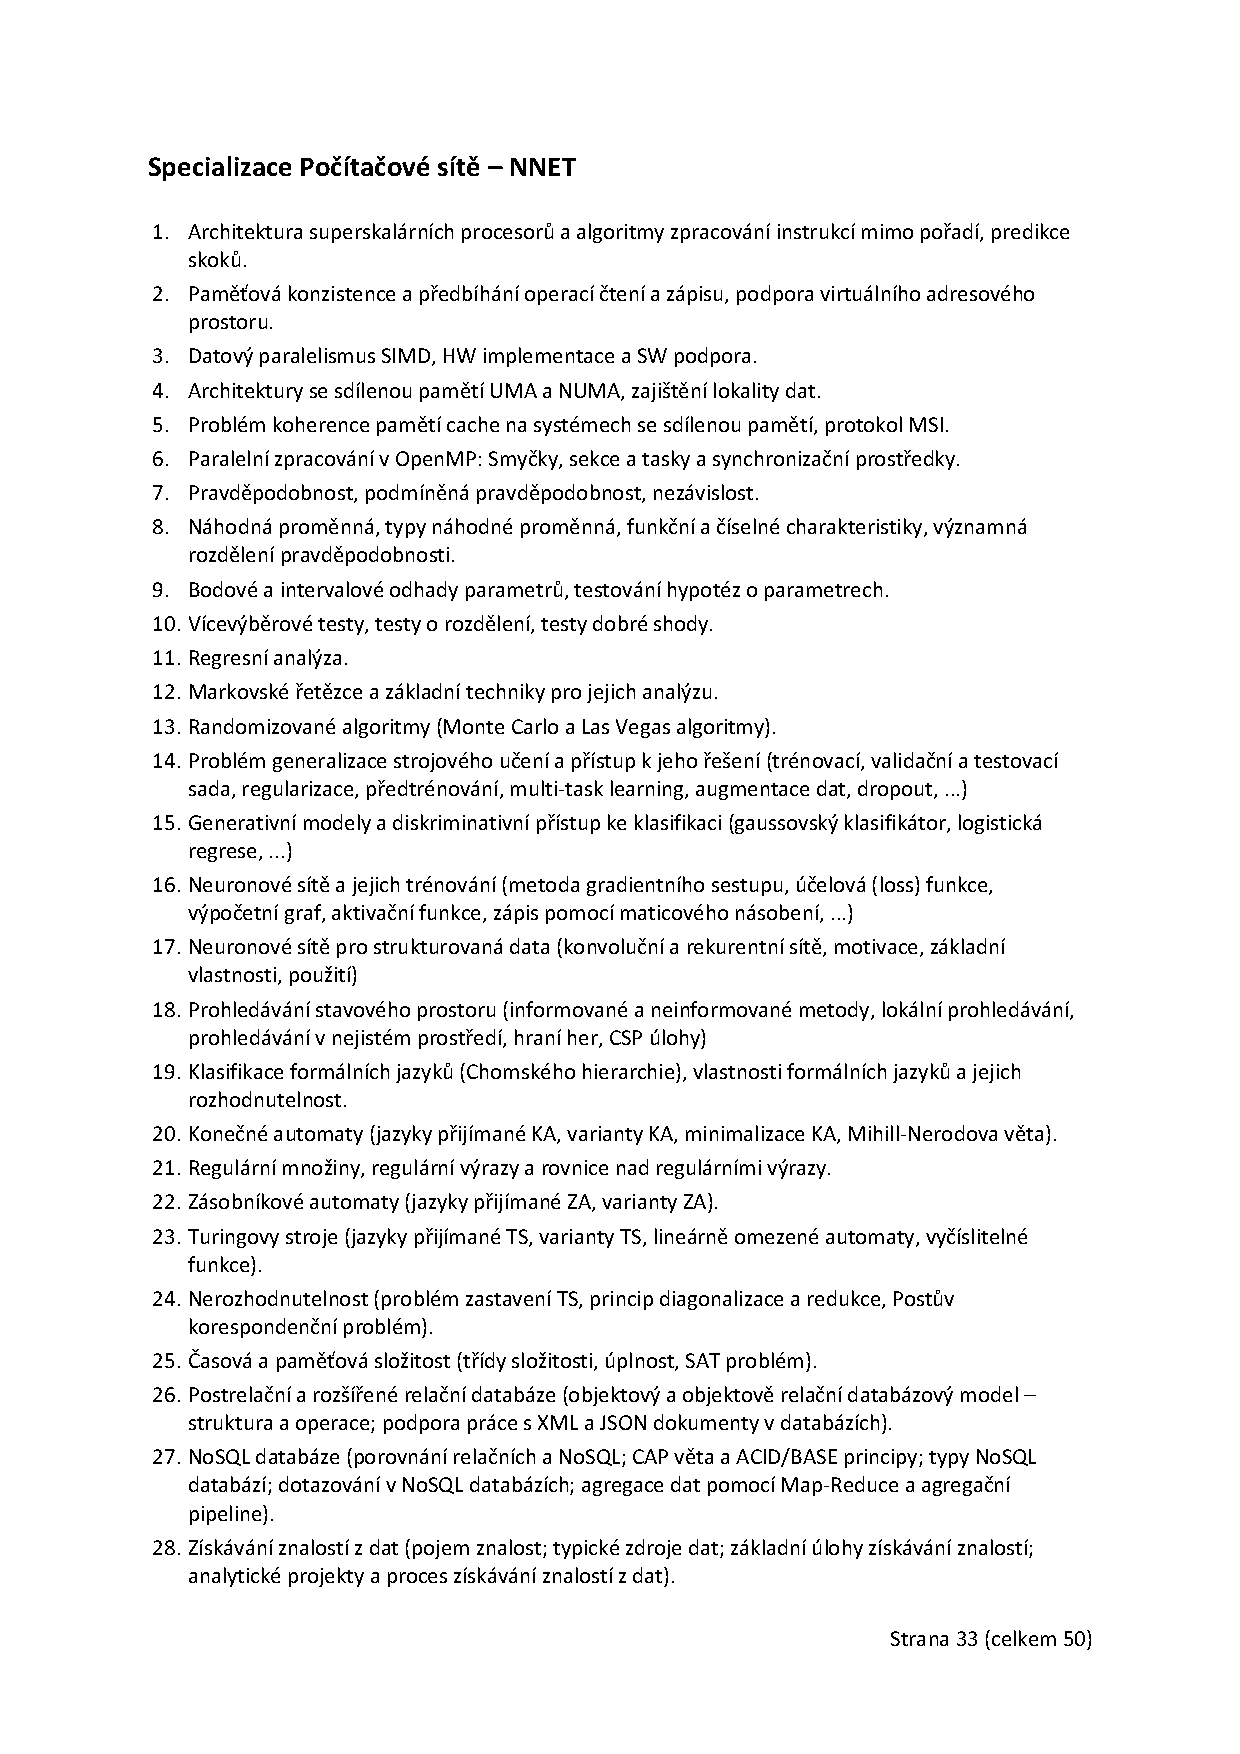
\includepdf[pages=-]{statnicovy_otazky_2022_nnet.pdf}

%%%%%%%%%%%%%%%%%%%%%%%%%%%%%%%%%%%%%%%%%%%%%%%%%%%%%%%%%%%%%%%%%%%%%%%%%%%%%%%%

\tableofcontents
\newpage

%%%%%%%%%%%%%%%%%%%%%%%%%%%%%%%%%%%%%%%%%%%%%%%%%%%%%%%%%%%%%%%%%%%%%%%%%%%%%%%%

% VUT FIT MITAI
% MSZ 2021/2022
% Author: Vladimir Dusek
% Login: xdusek27

%%%%%%%%%%%%%%%%%%%%%%%%%%%%%%%%%%%%%%%%%%%%%%%%%%%%%%%%%%%%%%%%%%%%%%%%%%%%%%%%

\chapter{Hledání minimální kostry obyčejného grafu (pojmy, stromy a kostry, Kruskalův algoritmus, Primův algoritmus).}

%%%%%%%%%%%%%%%%%%%%%%%%%%%%%%%%%%%%%%%%%%%%%%%%%%%%%%%%%%%%%%%%%%%%%%%%%%%%%%%%

\section{Metadata}

\begin{itemize}
    \item Předmět: Grafové algoritmy (GAL)
    \item Přednáška:
    \begin{itemize}
        \item 5) Stromy, minimální kostry, Jarníkův a Borůvkův algoritmus.
        \item 6) Růst minimální kostry, algoritmy Kruskala a Prima.
    \end{itemize}
    \item Záznam:
    \begin{itemize}
        \item 2020-10-22
        \item 2020-10-29
    \end{itemize}
\end{itemize}

%%%%%%%%%%%%%%%%%%%%%%%%%%%%%%%%%%%%%%%%%%%%%%%%%%%%%%%%%%%%%%%%%%%%%%%%%%%%%%%%

\section{Úvod a kontext}

\paragraph*{Orientovaný graf} Orientovaný graf je dvojice $G = (V, E)$, kde $V$ je konečná množina uzlů a $E \subseteq V \times V$ je množina hran.

\paragraph*{Neorientovaný graf} Neorientovaný graf je dvojice $G = (V, E)$, kde $V$ je konečná množina uzlů a $E \subseteq \binom{V}{2}$ je množina hran. (Hrana je tedy dvouprvková množina, avšak běžně se držíme stejného značení jako u orientovaných grafů a používáme dvojici.)

\paragraph*{Ohodnocený graf} Ohodnocený graf je takový graf, jehož každá hrana má přiřazenou nějakou hodnotu, typicky definovanou pomocí váhové funkce $w : E \mapsto \mathbb{R}$.

\paragraph*{Podgraf} Graf $G' = (V', E')$ je podgraf grafu $G = (V, E)$ jestliže $V' \subseteq V$ a $E' \subseteq E$.

\paragraph*{Sled} Posloupnost uzlů $\langle v_0, v_1, \dots, v_k \rangle$, kde $(v_{i-1}, v_i) \in E$ pro $i = 1, \dots, k$ se nazývá sled délky $k$ z $v_0$ do $v_k$.

\paragraph*{Uzavřený sled} Sled $\langle v_0, v_1, \dots, v_k \rangle$ se nazývá uzavřený, pokud existuje hrana $(v_0, v_k)$.

\paragraph*{Dosažitelnost} Pokud existuje sled $s$ z uzlu $u$ do uzlu $v$, říkáme, že $v$ je dosažitelný z $u$ sledem $s$, značeno $u \xRightarrow{\text{s}} v$.

\paragraph*{Tah} Tah je sled ve kterém se neopakují hrany.

\paragraph*{Cesta} Cesta je sled ve kterém se neopakují uzly.

\paragraph*{Souvislý graf} Neorientovaný graf se nazývá souvislý, pokud mezi libovolnými dvěma uzly existuje cesta.

\paragraph*{Kružnice} Uzavřená cesta se nazývá kružnice.

\paragraph*{Cyklus} Orientovaná kružnice se nazývá cyklus (první a poslední uzel je shodný).

\paragraph*{Prostý graf} Orientovaný graf bez cyklů se nazývá prostý.

\paragraph*{Acyklický graf} Graf je bez cyklů, resp. kružnic, se nazývá acyklický.

\paragraph*{Strom} Graf, který je souvislý a acyklický, se nazývá strom.

\paragraph*{Kostra} Strom, který tvoří podgraf souvislého grafu na množině všech jeho vrcholů, se nazývá kostra (\textit{spanning tree}).

\paragraph*{Minimální kostra} Nechť $G = (V, E)$ je souvislý neorientovaný graf s váhovou funkcí $w : E \mapsto \mathbb{R}$. Minimální kostra (\textit{MST, minimum spanning tree}) je strom $G' = (V, E')$, kde $E' \subseteq E$ a $$w(E') = \sum_{(u,v) \in T} w(u, v)$$ je minimální ze všech možných alternativních koster.

\paragraph*{Seznam sousedů} Seznam sousedů (Adj, \textit{adjacency list}) je reprezentace grafu v paměti. Jde o preferovanou variantu pro řídké grafy~--~kde $m << n^2$. Pro každý uzel máme definovaný seznam jeho sousedů.

\paragraph*{Matice sousednosti} Matice sousednosti (\textit{adjacency matrix}) je reprezentace grafu v paměti. Jde o preferovanou variantu pro husté grafy~--~kde $m$ je skoro $n^2$.

\begin{figure}[H]
    \centering
    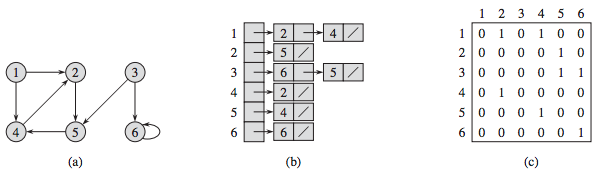
\includegraphics[width=1\linewidth]{45/graph_representations_example.png}
    \caption{Příklad reprezentace grafu pomocí seznamu sousedů a matice sousednosti.}
\end{figure}

%%%%%%%%%%%%%%%%%%%%%%%%%%%%%%%%%%%%%%%%%%%%%%%%%%%%%%%%%%%%%%%%%%%%%%%%%%%%%%%%

\section{Generický algoritmus}

Hledání minimální kostry je problém, který lze řešit algoritmy, které spadají do kategorie tzv. hladových (\textit{greedy}) deterministických algoritmů. Spočívají v tom, že průběžně odhadují kostru přidáváním dalších hran a nikdy se nemusejí vracet (neprovádí se \textit{backtracking}).

\bigskip

\noindent Generický algoritmus tvoří jakousi základní kostru pro další, už konkrétní, algoritmy.

\paragraph*{Řez} Nechť $G = (V, E)$ je graf. Řez grafu $G$ je dvojice $(S, V - S)$, kde $\emptyset \subseteq S \subseteq V$.

\paragraph*{Křížení} Hrana $(u, v) \in E$ kříží řez $(S, V - S)$, pokud jeden její konec je v $S$ a druhý v $V - S$.

\paragraph*{Respektování} Nechť $A \subseteq E$ je množina hran. Řez $(S, V - S)$ respektuje množinu hran $A$, pokud žádná hrana v $A$ nekříží řez $(S, V - S)$.

\paragraph*{Lehkost} Nechť $(S, V - S)$ je řez a $B$ je množina hran, která ho kříží. Hrana z množiny $B$ s nejmenší hodnotou se nazývá lehká.

\paragraph*{Bezpečnost} Nechť $G = (V, E)$ je souvislý neorientovaný graf s reálnou váhovou funkcí $w$. Nechť $A \subseteq E$ je součástí nějaké minimální kostry $G$. Nechť $(S, V - S)$ je řez, který respektuje $A$. Nechť $(u, v)$ je lehká hrana křížící $(S, V - S)$. Pak hrana $(u, v)$ je bezpečná pro $A$.

\bigskip\noindent\begin{minipage}{\linewidth}
\begin{lstlisting}[language=Python, caption={Generický algoritmus. Před každou iterací algoritmu je množina $A$ podmnožinou nějaké minimální kostry. Hrana $(u,v) \in E$ je bezpečná pro $A$, pokud $A \cup \{(u, v)\}$ je podmnožinou nějaké minimální kostry.}]
def generic_mst(G):
    # G je graf
    # A je mnozina hran rozpracovane minimalni kostry
    A = {}
    while netvori_kostru(A, G):
        for hrana in G.E:
            if je_bezpecna(A, hrana):
                A += {hrana}
    return A
\end{lstlisting}
\end{minipage}

\begin{figure}[H]
    \centering
    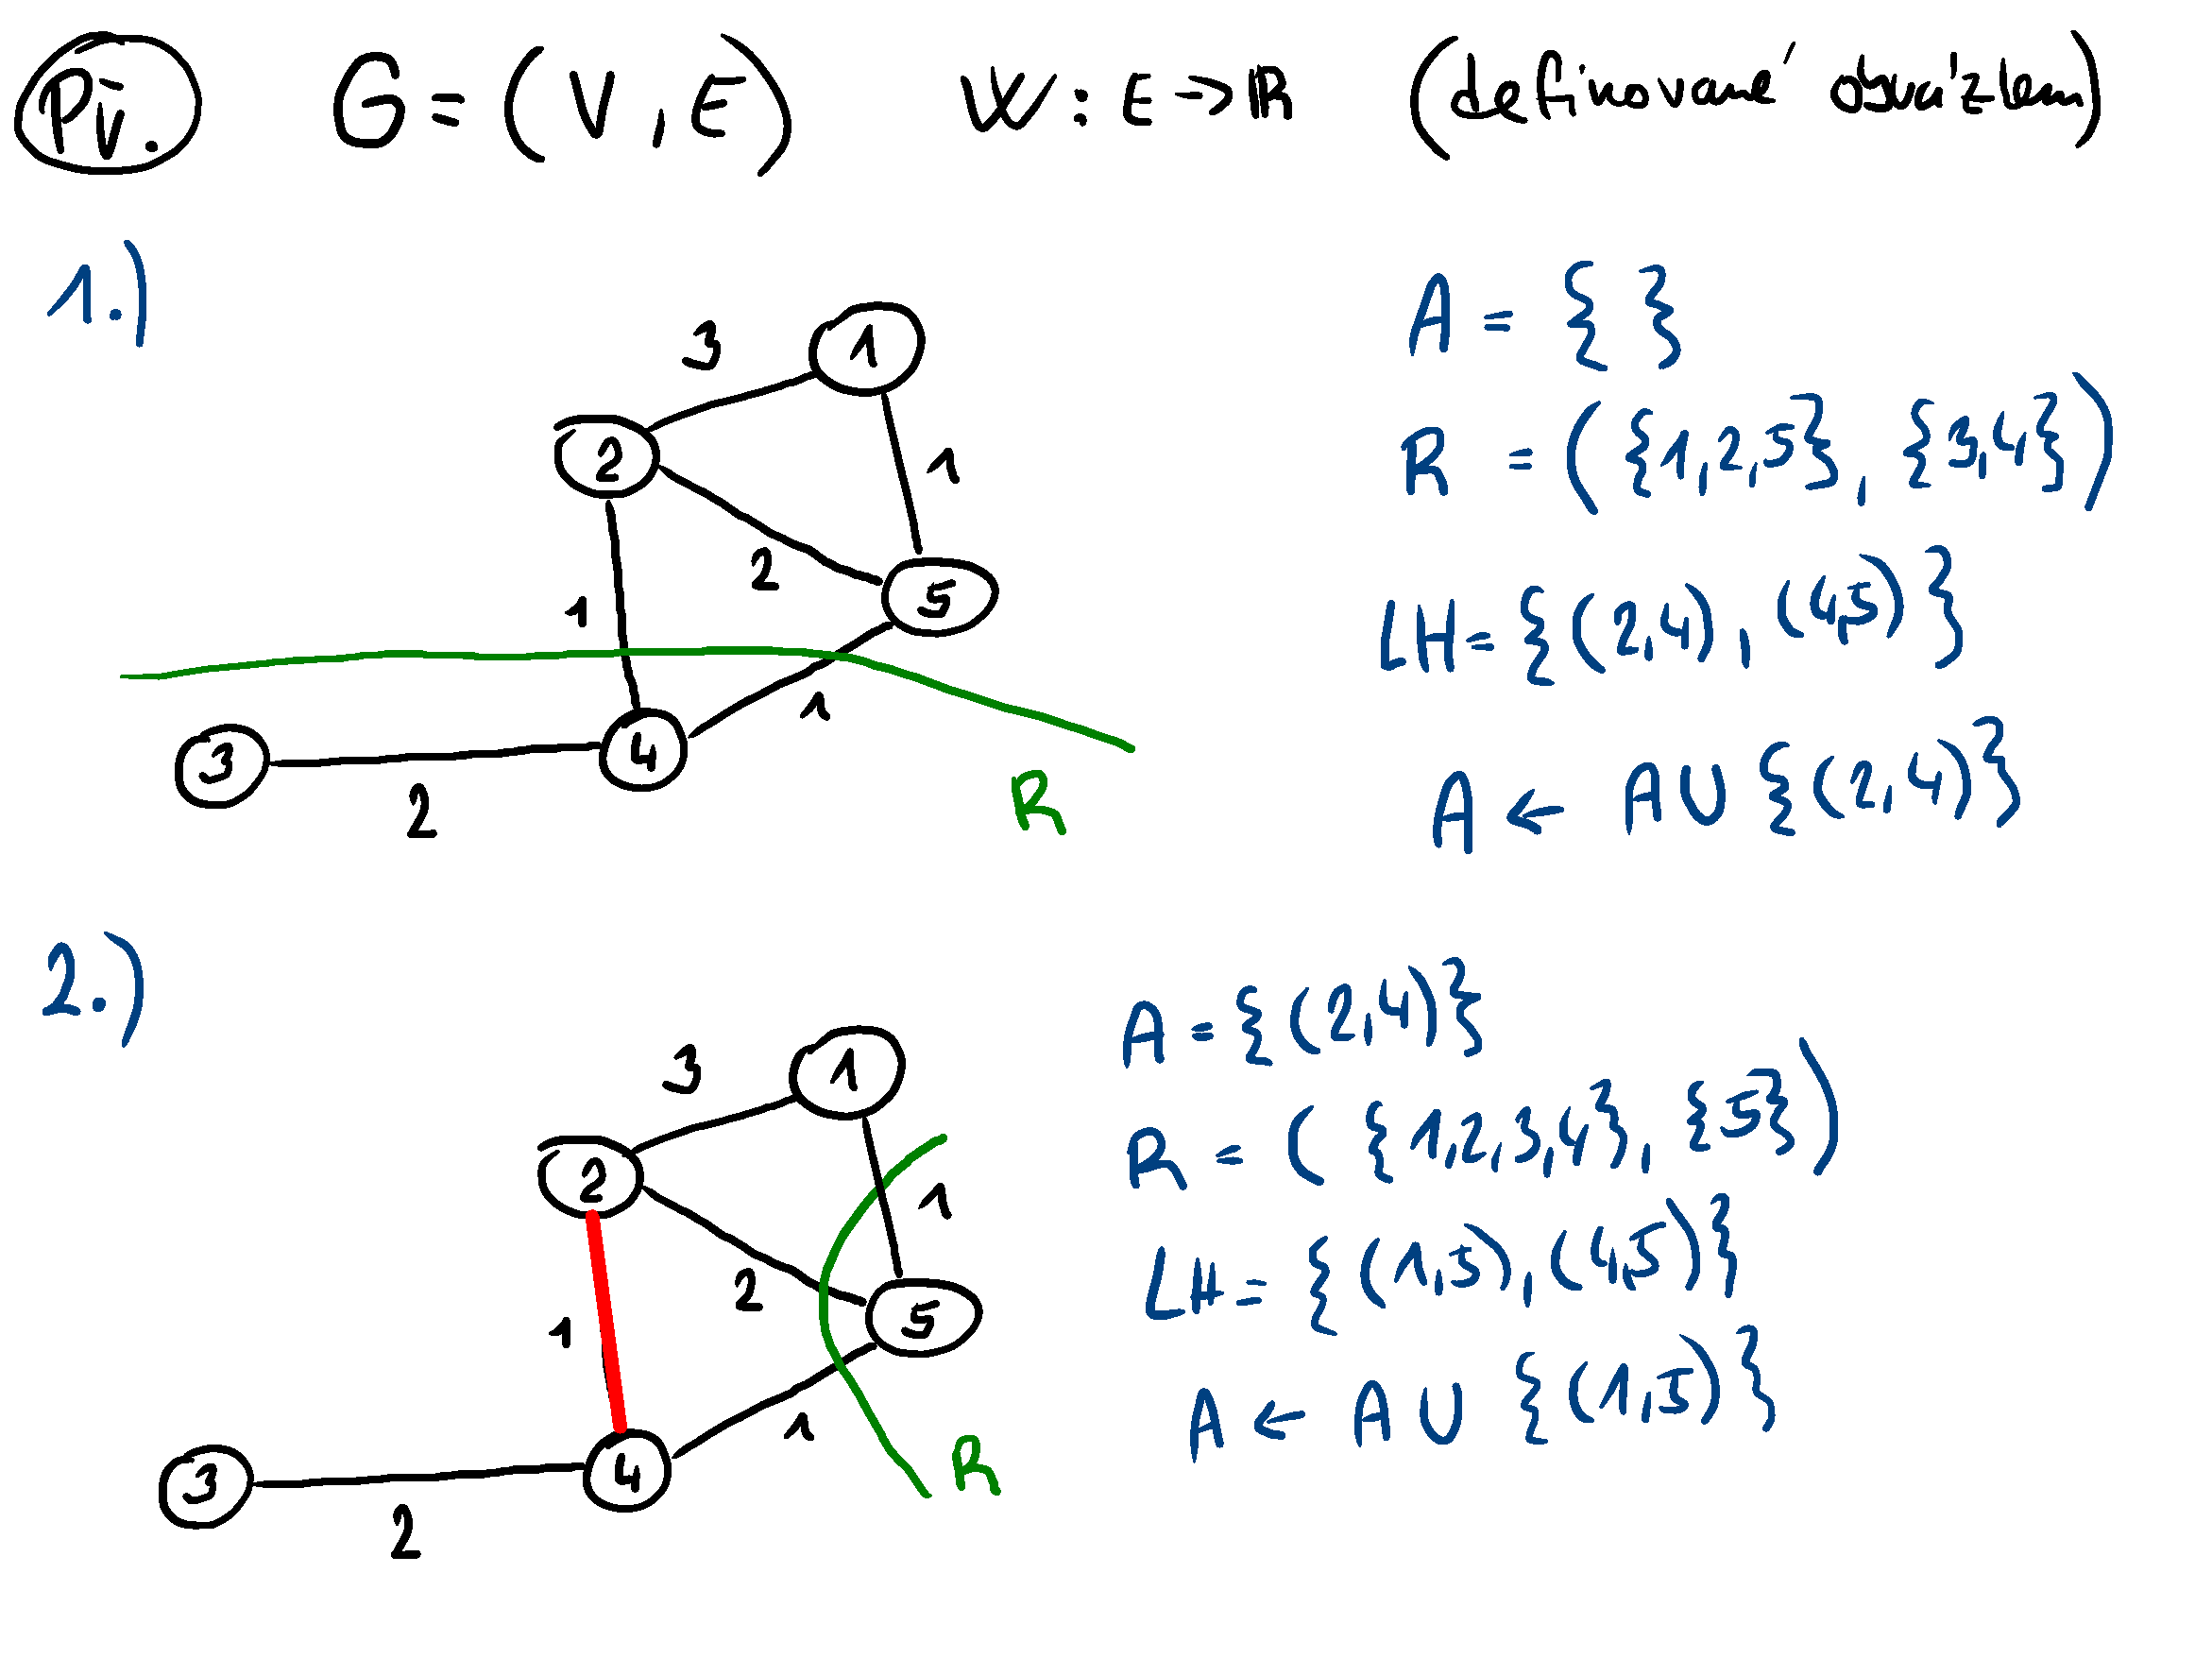
\includegraphics[width=0.9\linewidth]{45/03-minimalni-kostry-6.pdf}
    \caption{Příklad, část 1.}
\end{figure}

\begin{figure}[H]
    \centering
    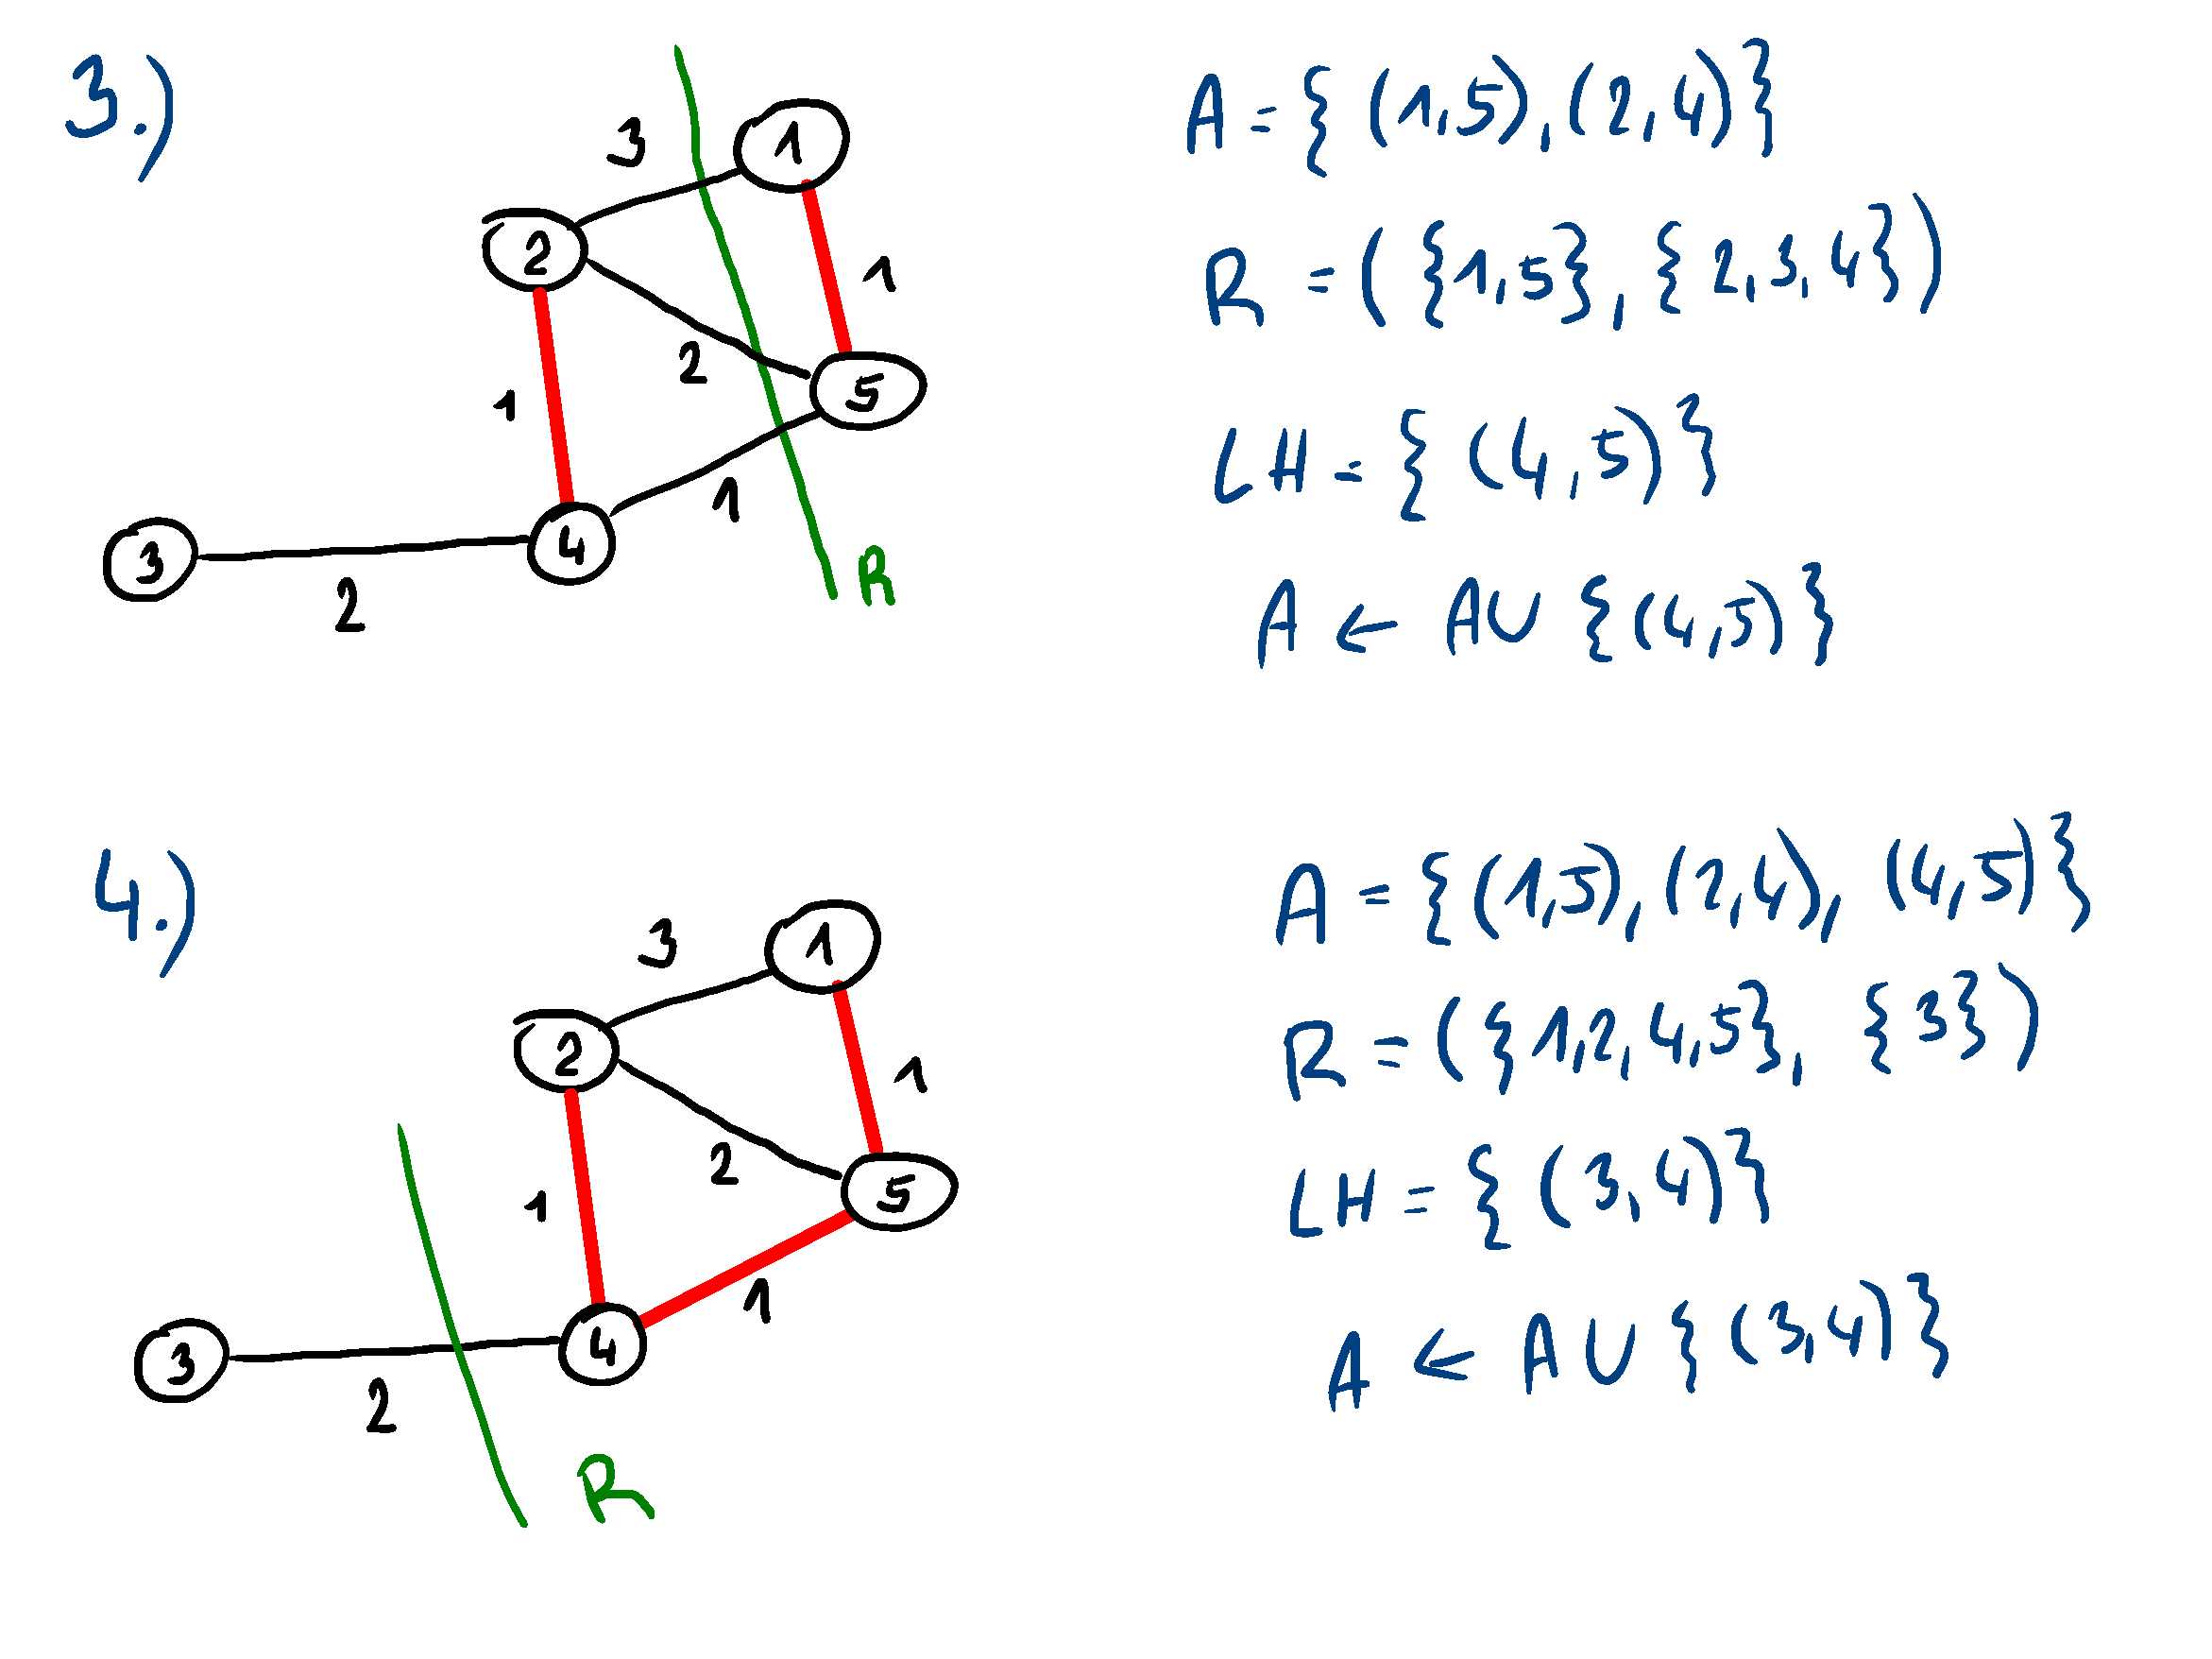
\includegraphics[width=0.9\linewidth]{45/03-minimalni-kostry-7.pdf}
    \caption{Příklad, část 2.}
\end{figure}

\begin{figure}[H]
    \centering
    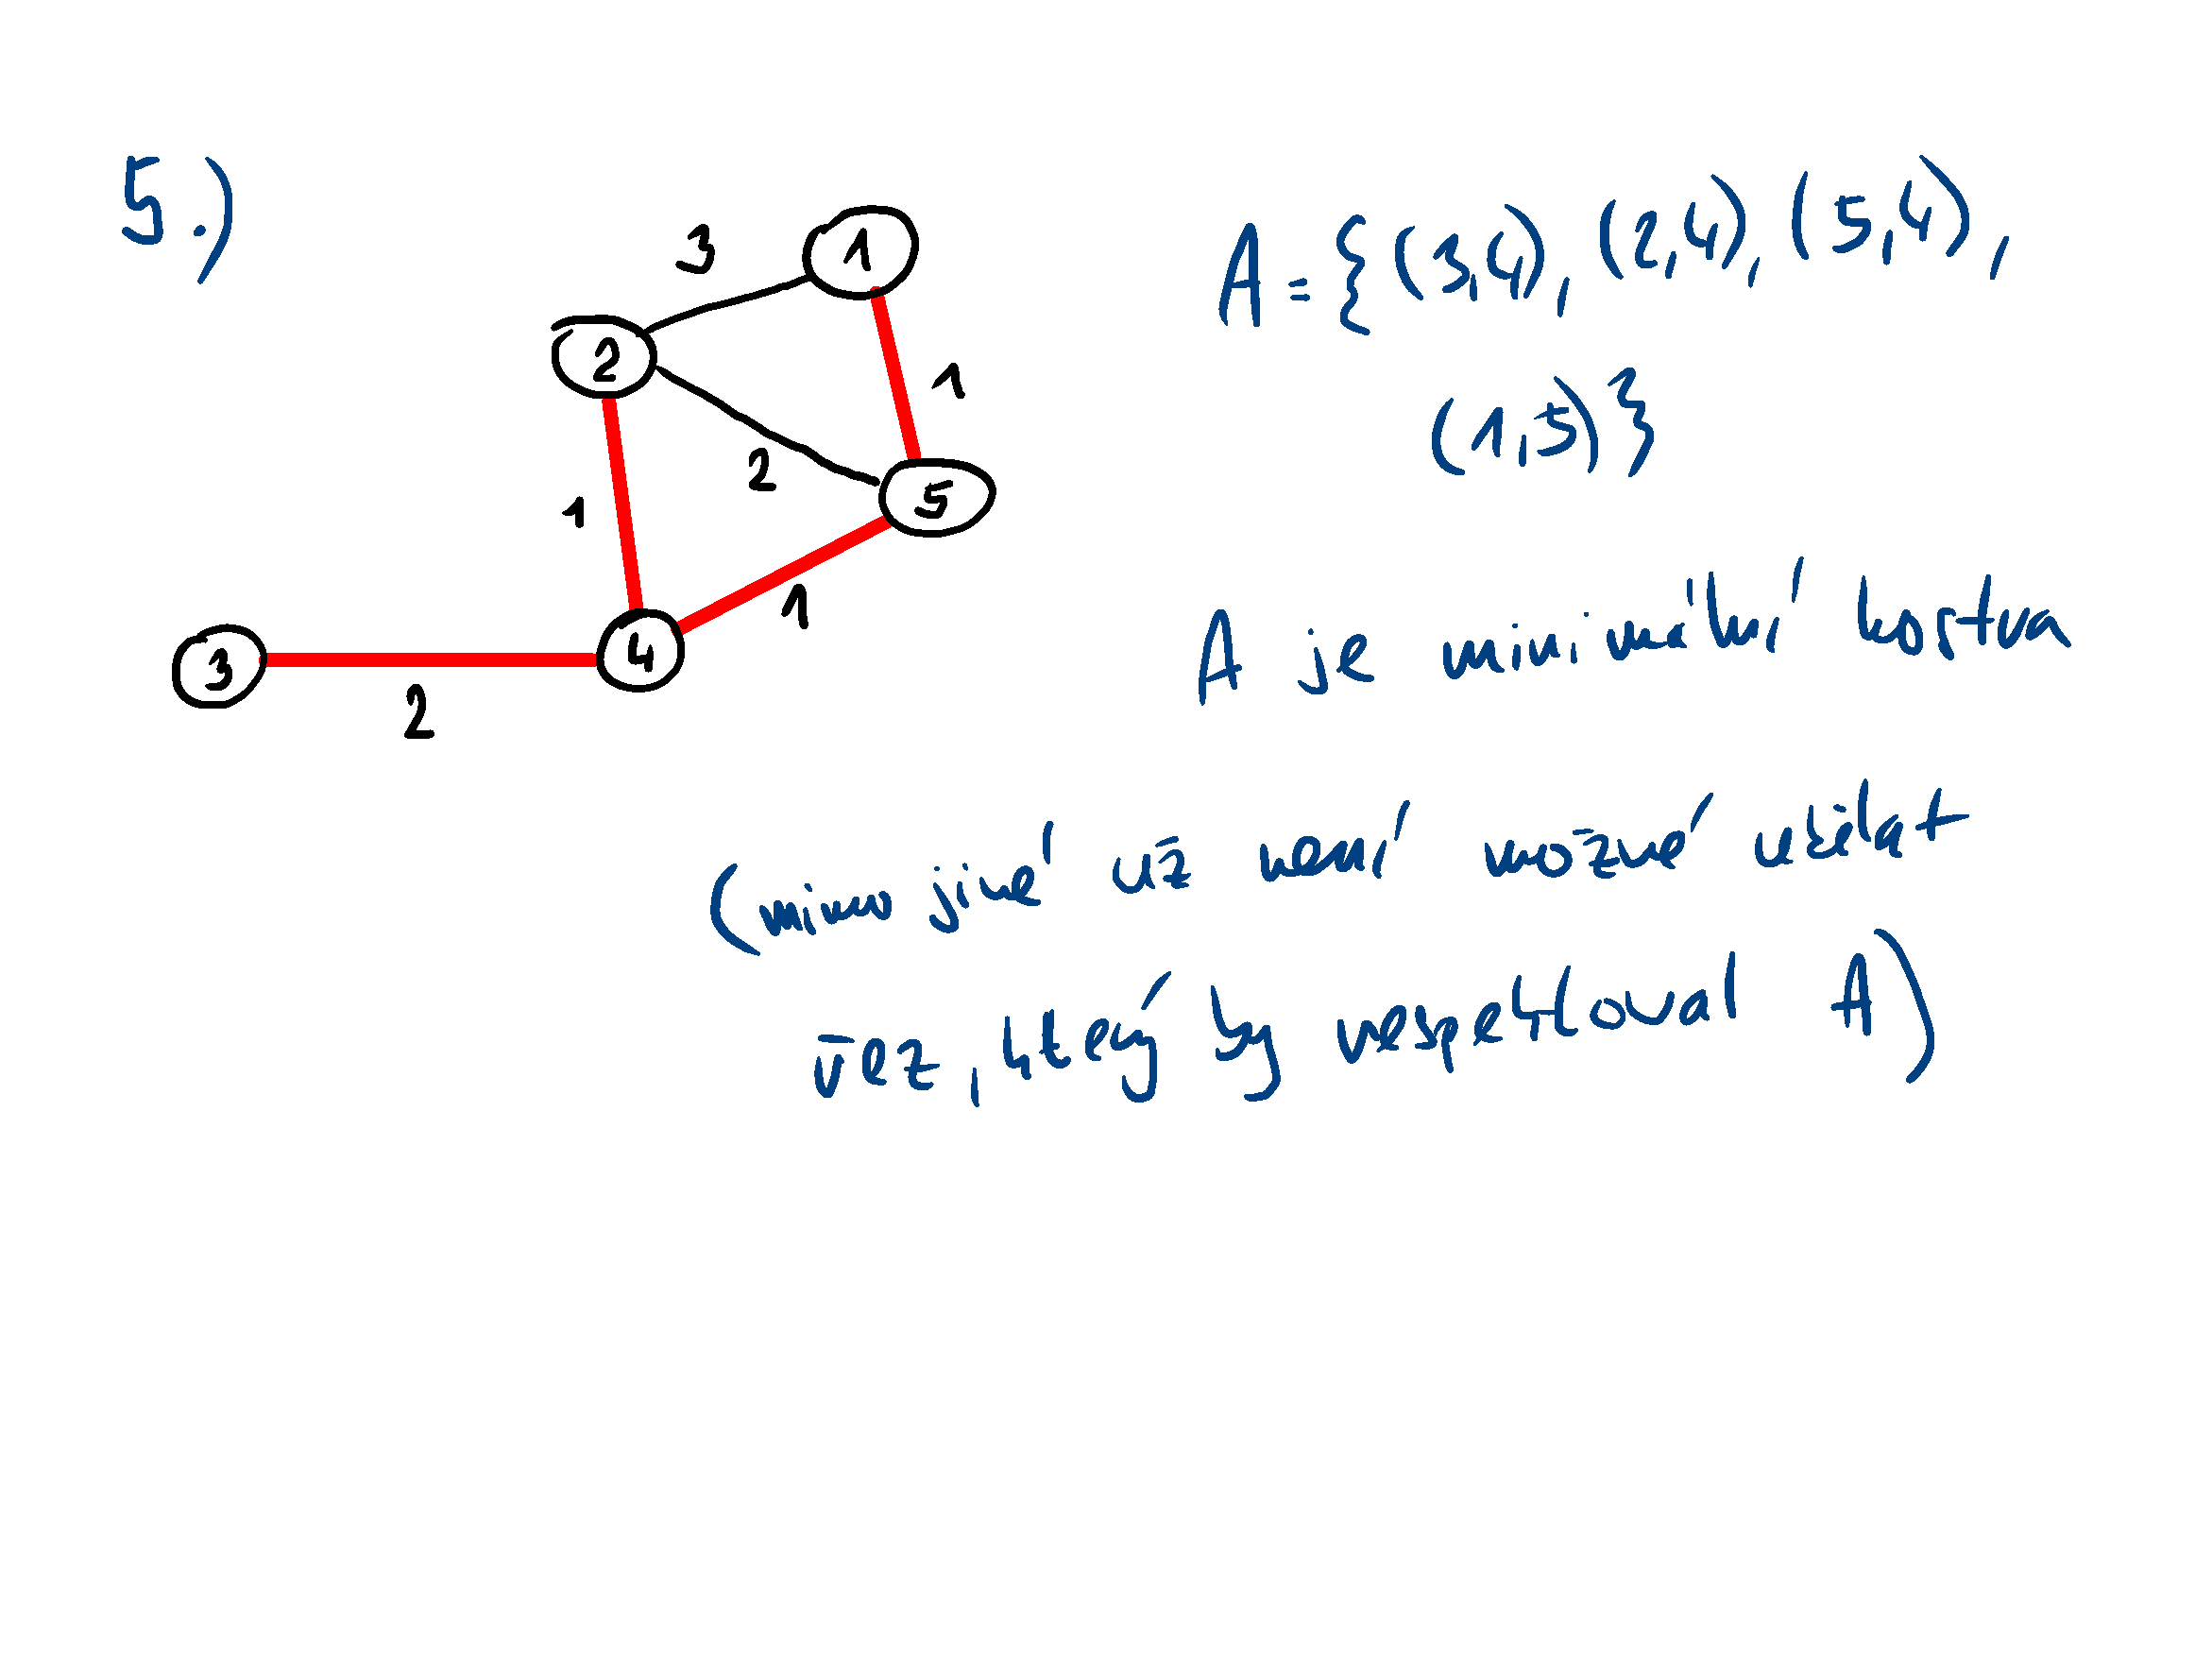
\includegraphics[width=0.9\linewidth]{45/03-minimalni-kostry-8.pdf}
    \caption{Příklad, část 3.}
\end{figure}

%%%%%%%%%%%%%%%%%%%%%%%%%%%%%%%%%%%%%%%%%%%%%%%%%%%%%%%%%%%%%%%%%%%%%%%%%%%%%%%%

\section{Kruskalův algoritmus}

Kruskalův a Primův algoritmus se liší v tom, jakým způsobem vybírají bezpečnou hranu. Kruskalův algoritmus nahlíží na $A$ jako na les a hledá hranu s nejmenším ohodnocením, která spojuje stromy v lese. Na konci je $A$ jeden strom.

\bigskip\noindent\begin{minipage}{\linewidth}
\begin{lstlisting}[language=Python, caption={Kruskalův algoritmus. Funkce \texttt{make\_set(v)} vytvoří množinu obsahující $v$, \texttt{find\_set} vrátí reprezentanta množiny $v$, \texttt{union(u ,v)} sjednotí dvě množiny obsahující $u$ a $v$.}]
def kruskal_mst(G):
    # G je graf
    # A je mnozina hran rozpracovane minimalni kostry

    # inicializace, kazdy uzel je ve sve mnozine
    A = {}
    for v in G.V:
        make_set(v)

    # seradit vzestupne podle w
    E = sort(G.E, G.w)

    for (u, v) in E:
        if find_set(u) != find_set(v):
            A += {(u, v)}
            union(u, v)

    return A
\end{lstlisting}
\end{minipage}

\subsection{Složitost}

\begin{itemize}
    \item Řádek 3 -- $O(1)$
    \item Řádek 6-7 -- $n$-krát složitost $make\_set$ ($n$ je počet uzlů).
    \item Řádek 10 -- $O(m \cdot \log(m))$ ($m$ je počet hran).
    \item Řádky 12-15 -- Závisí na implementaci $find\_set$ a $union$.
    \begin{itemize}
        \item Při implementaci seznamem s heuristickou celkem: $O(m + n \cdot \log(n))$.
        \item Při stromové implementaci s váhami a zkratkami celkem: $O((m+n) \cdot \alpha(n))$. Kde $\alpha$ je velmi pomalu rostoucí funkce ($\alpha \leq 4$).
    \end{itemize}
    \item Pro souvislý graf platí $m > n$. Proto množinové operace stojí $O(m \cdot \alpha(n))$. Jelikož $\alpha(n) = O(\log(n)) = O(\log(m))$, tak celková složitost je $O(m \cdot \log(m))$.
    \item Dále platí $m < n^2$, pak $\log(m) = O(\log(n))$, proto celkem: $O(m \cdot \log(n))$.
\end{itemize}

\subsection{Příklad}

\begin{figure}[H]
    \centering
    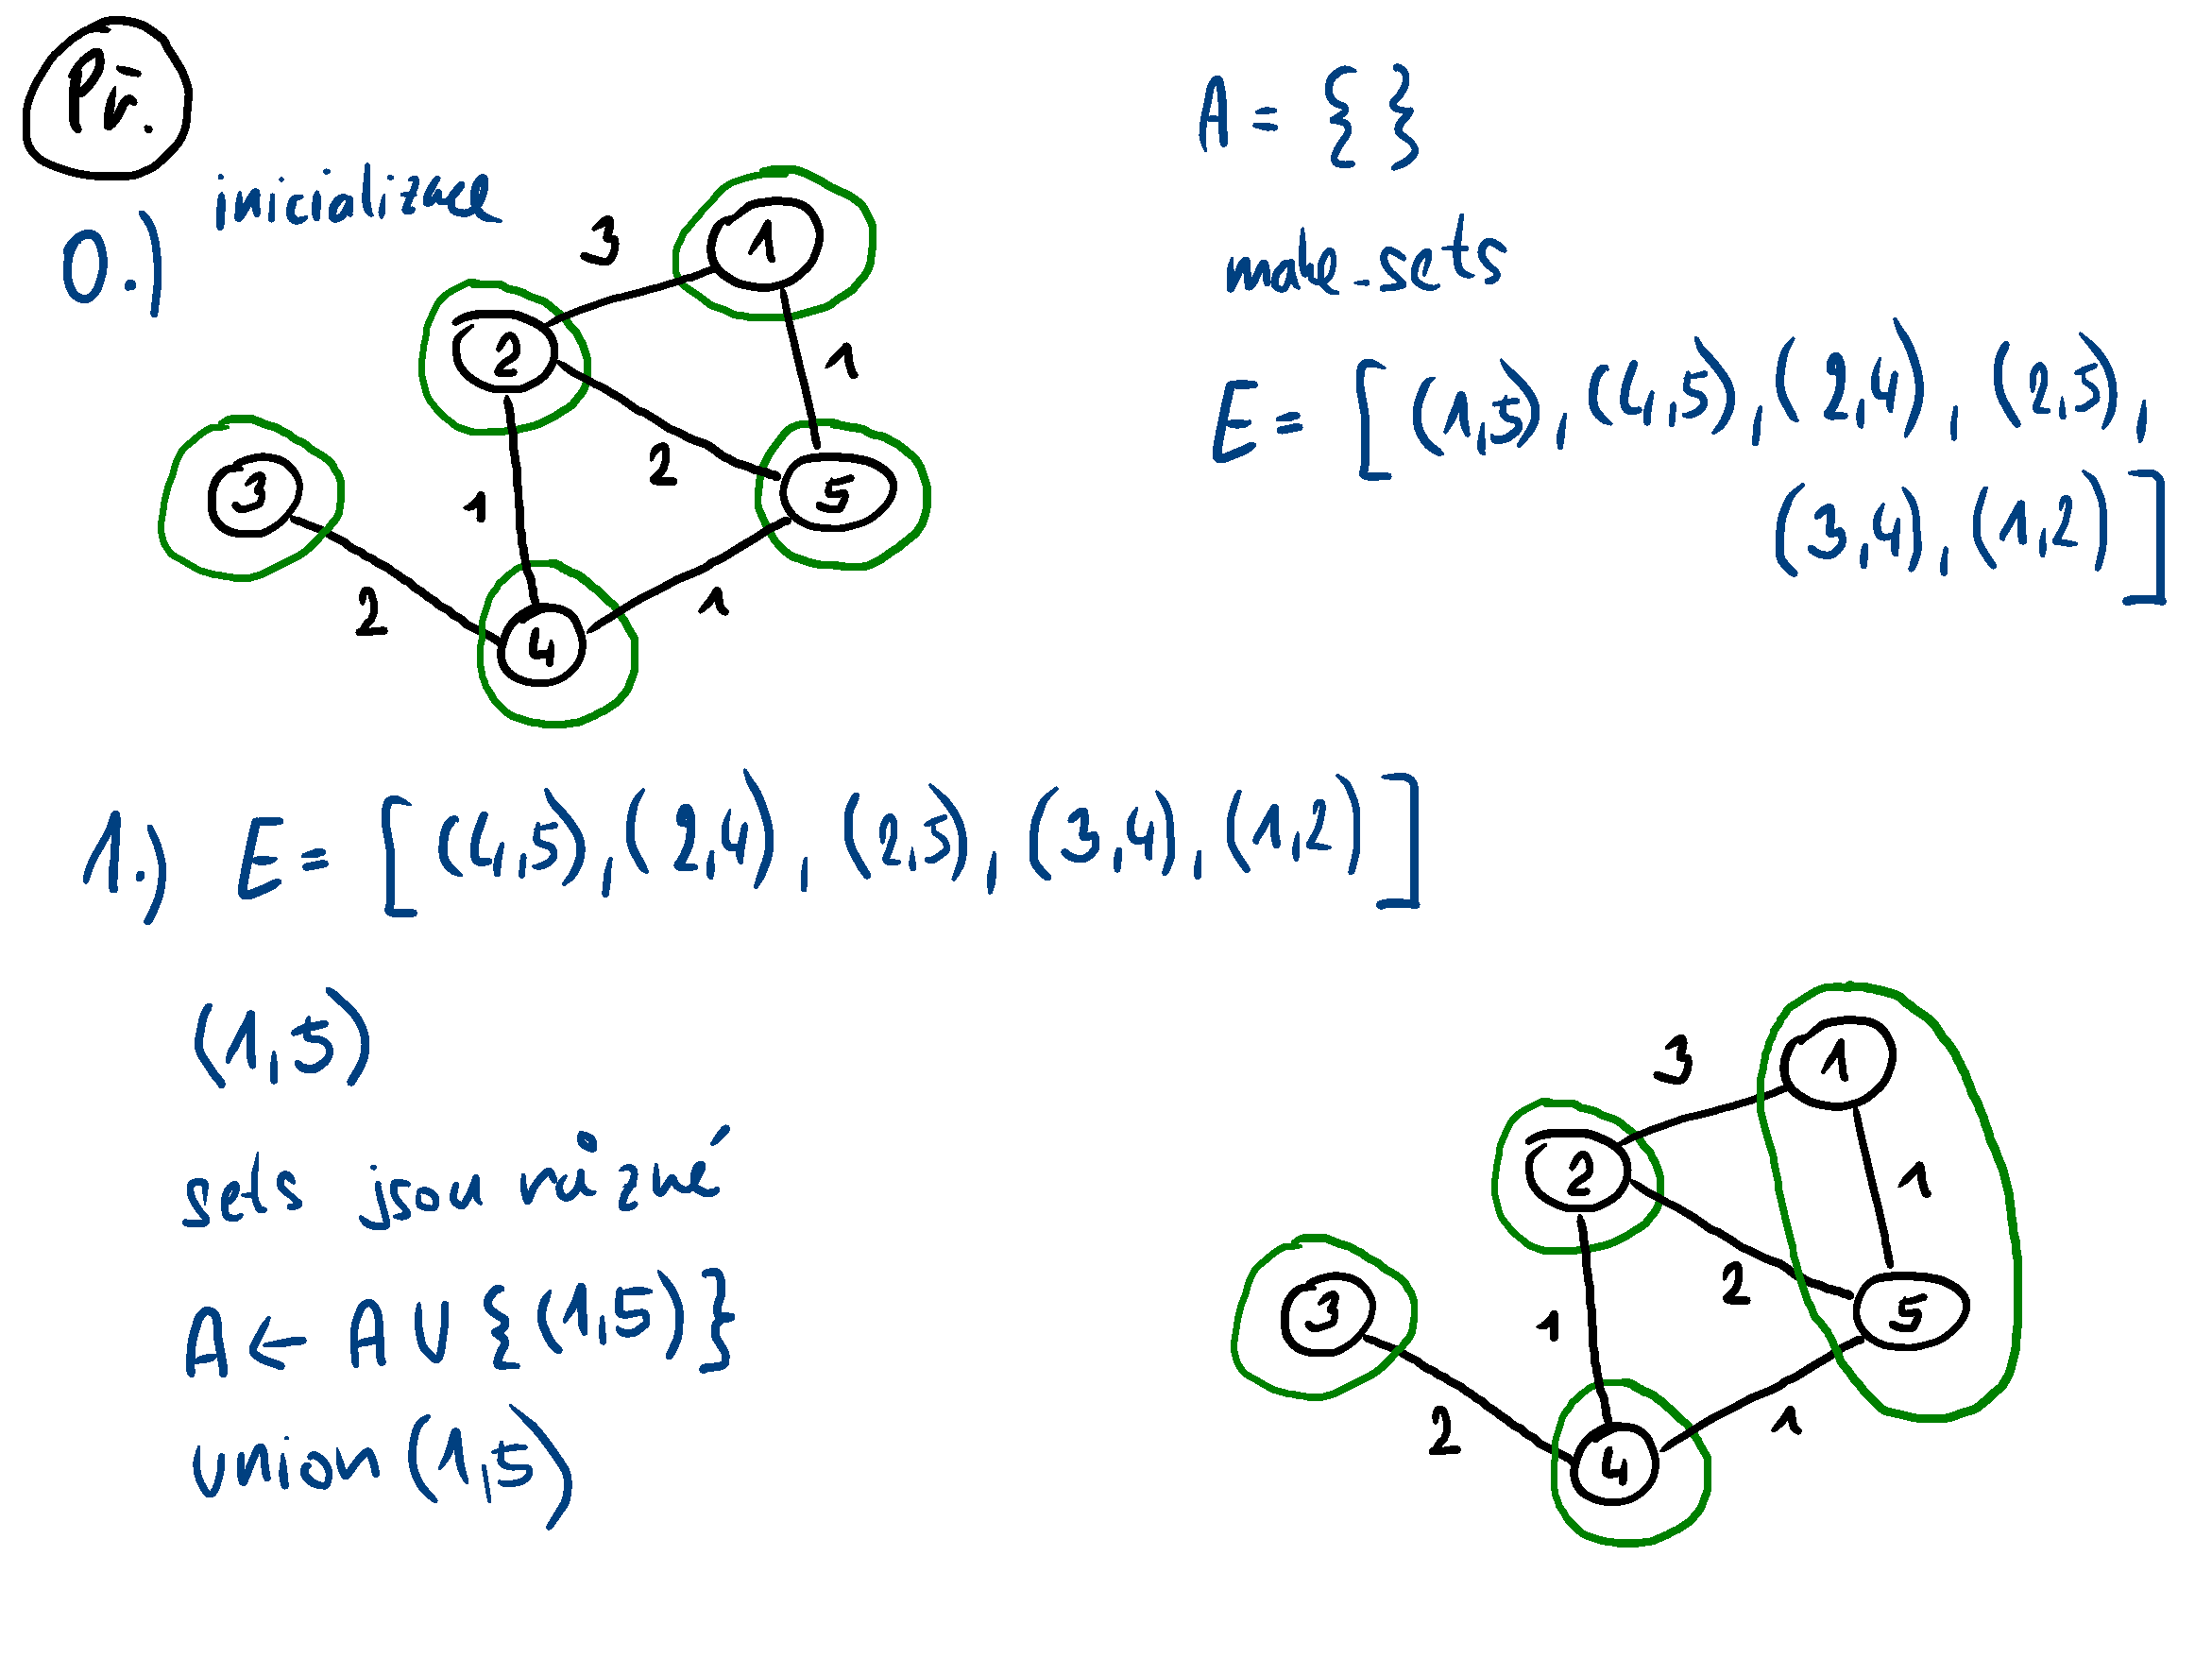
\includegraphics[width=0.9\linewidth]{45/03-minimalni-kostry-11.pdf}
    \caption{Příklad, část 1.}
\end{figure}

\begin{figure}[H]
    \centering
    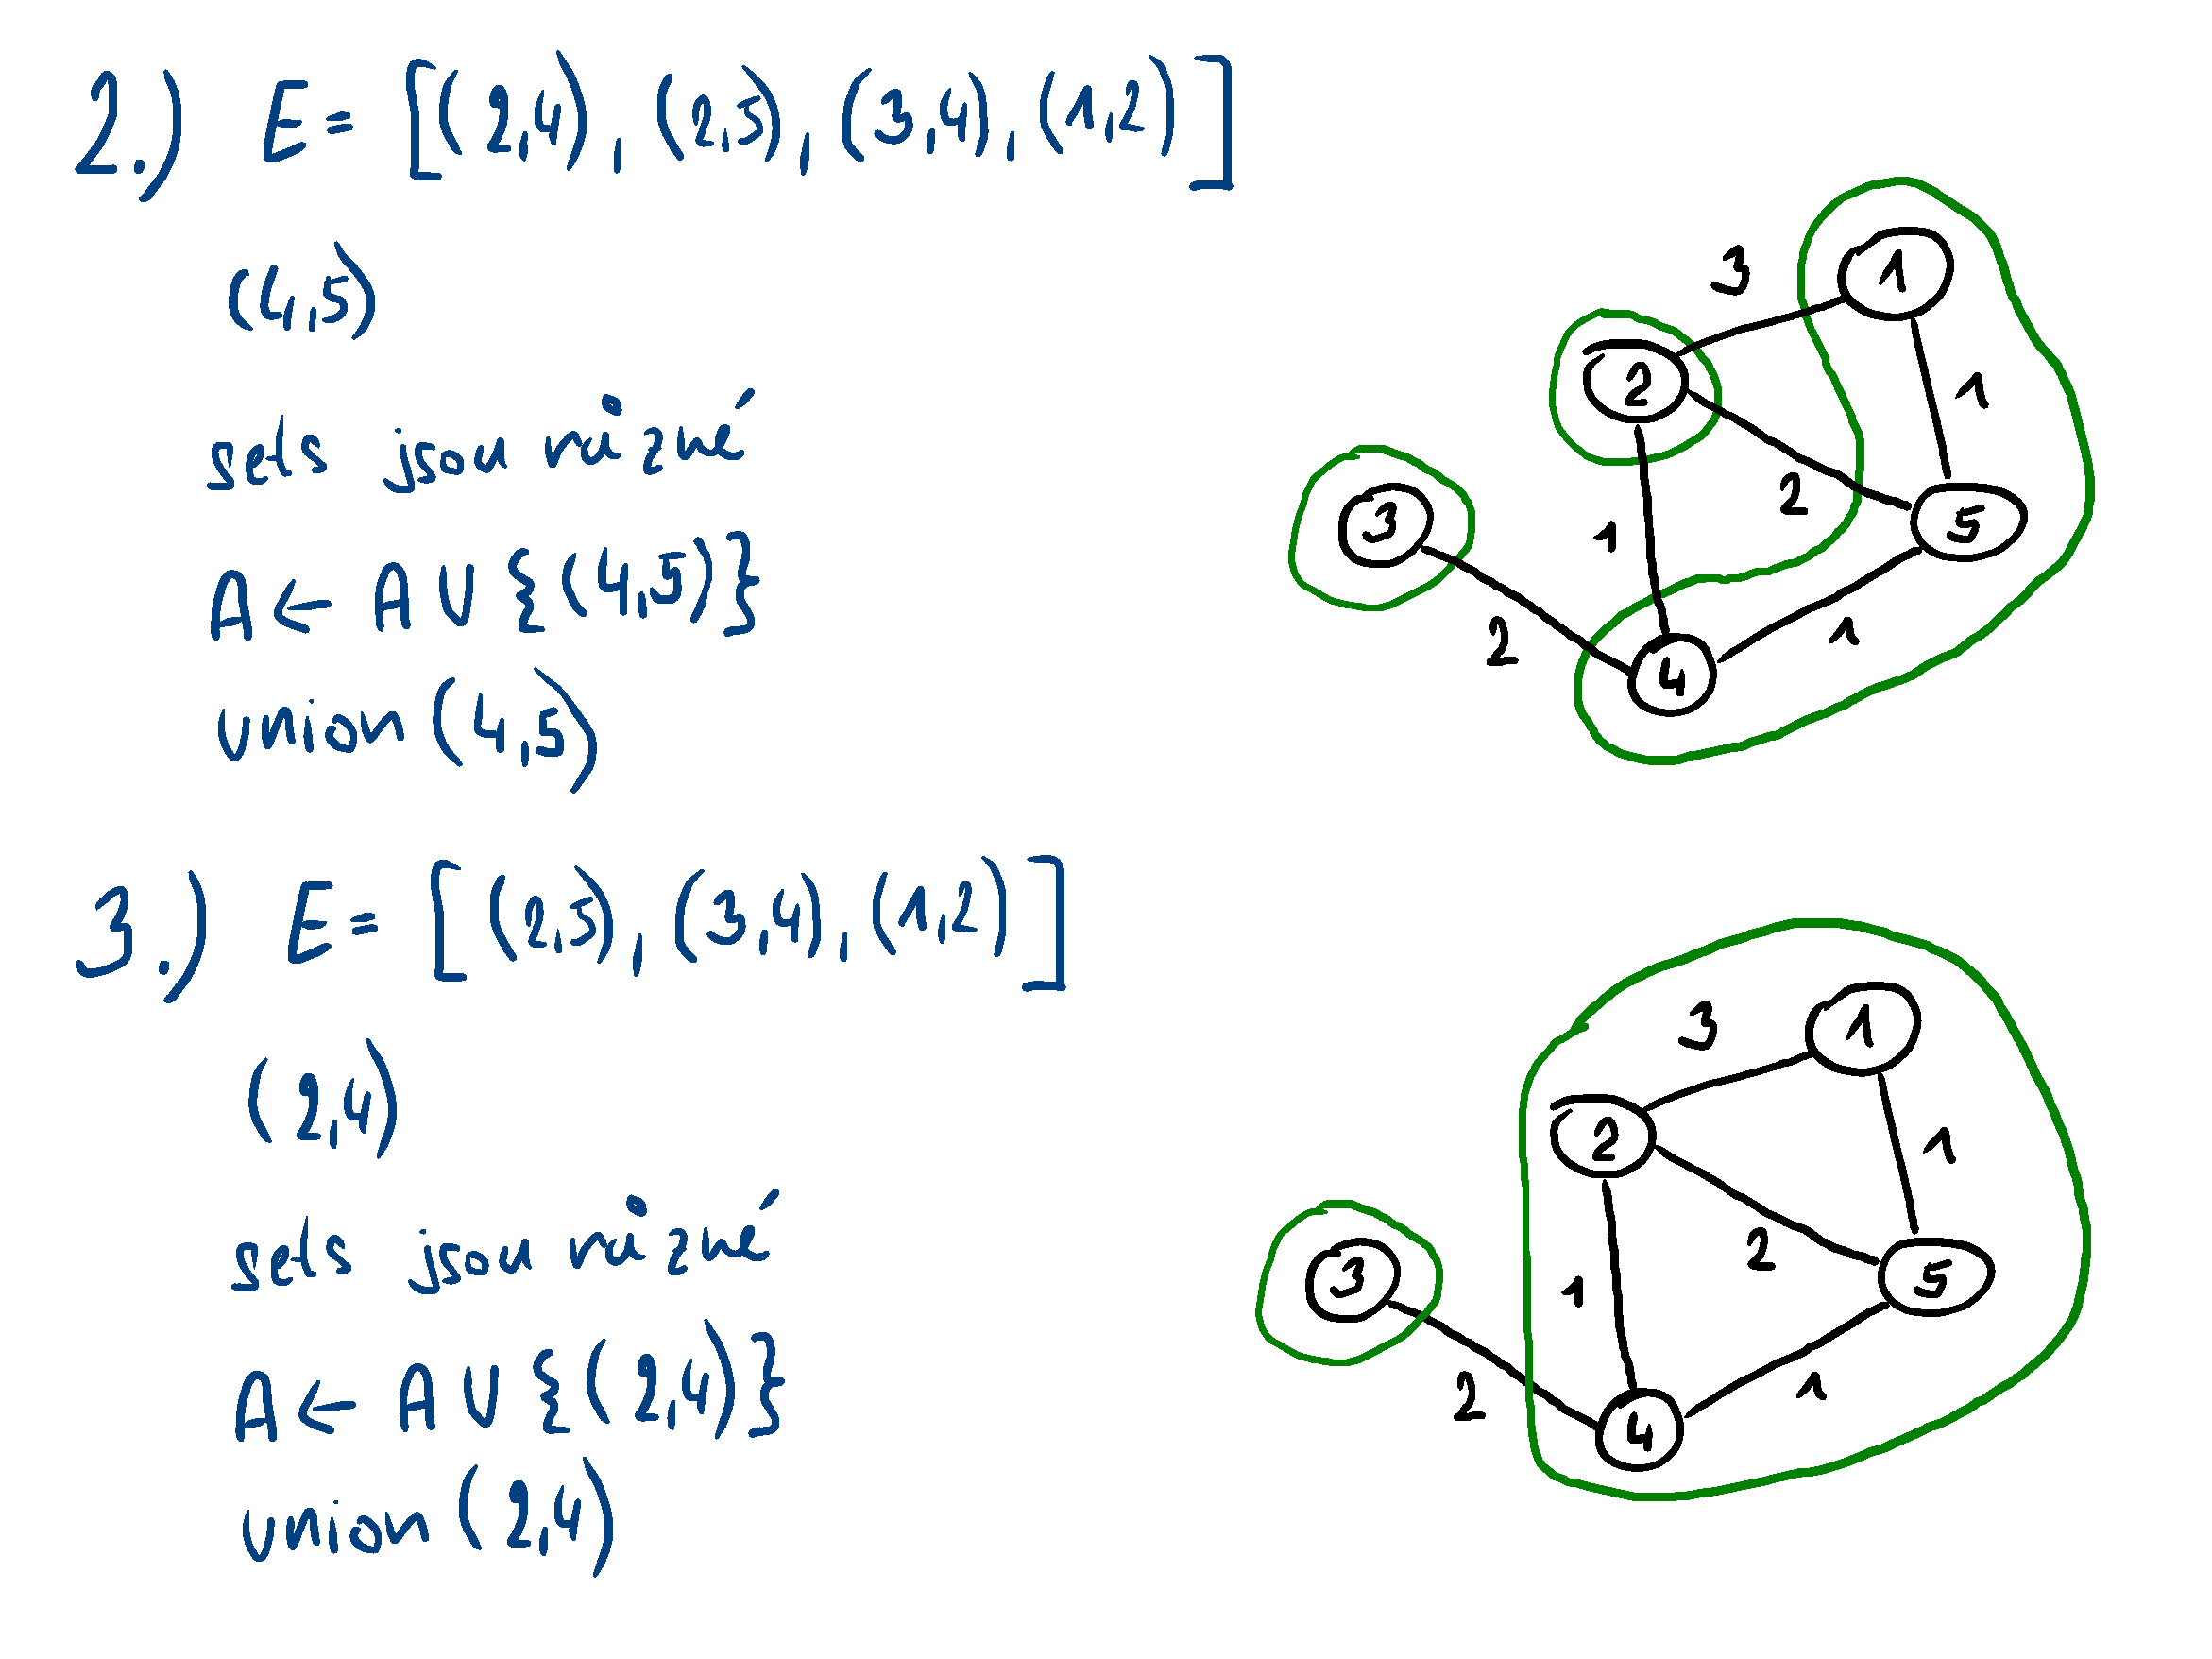
\includegraphics[width=0.9\linewidth]{45/03-minimalni-kostry-12.pdf}
    \caption{Příklad, část 2.}
\end{figure}

\begin{figure}[H]
    \centering
    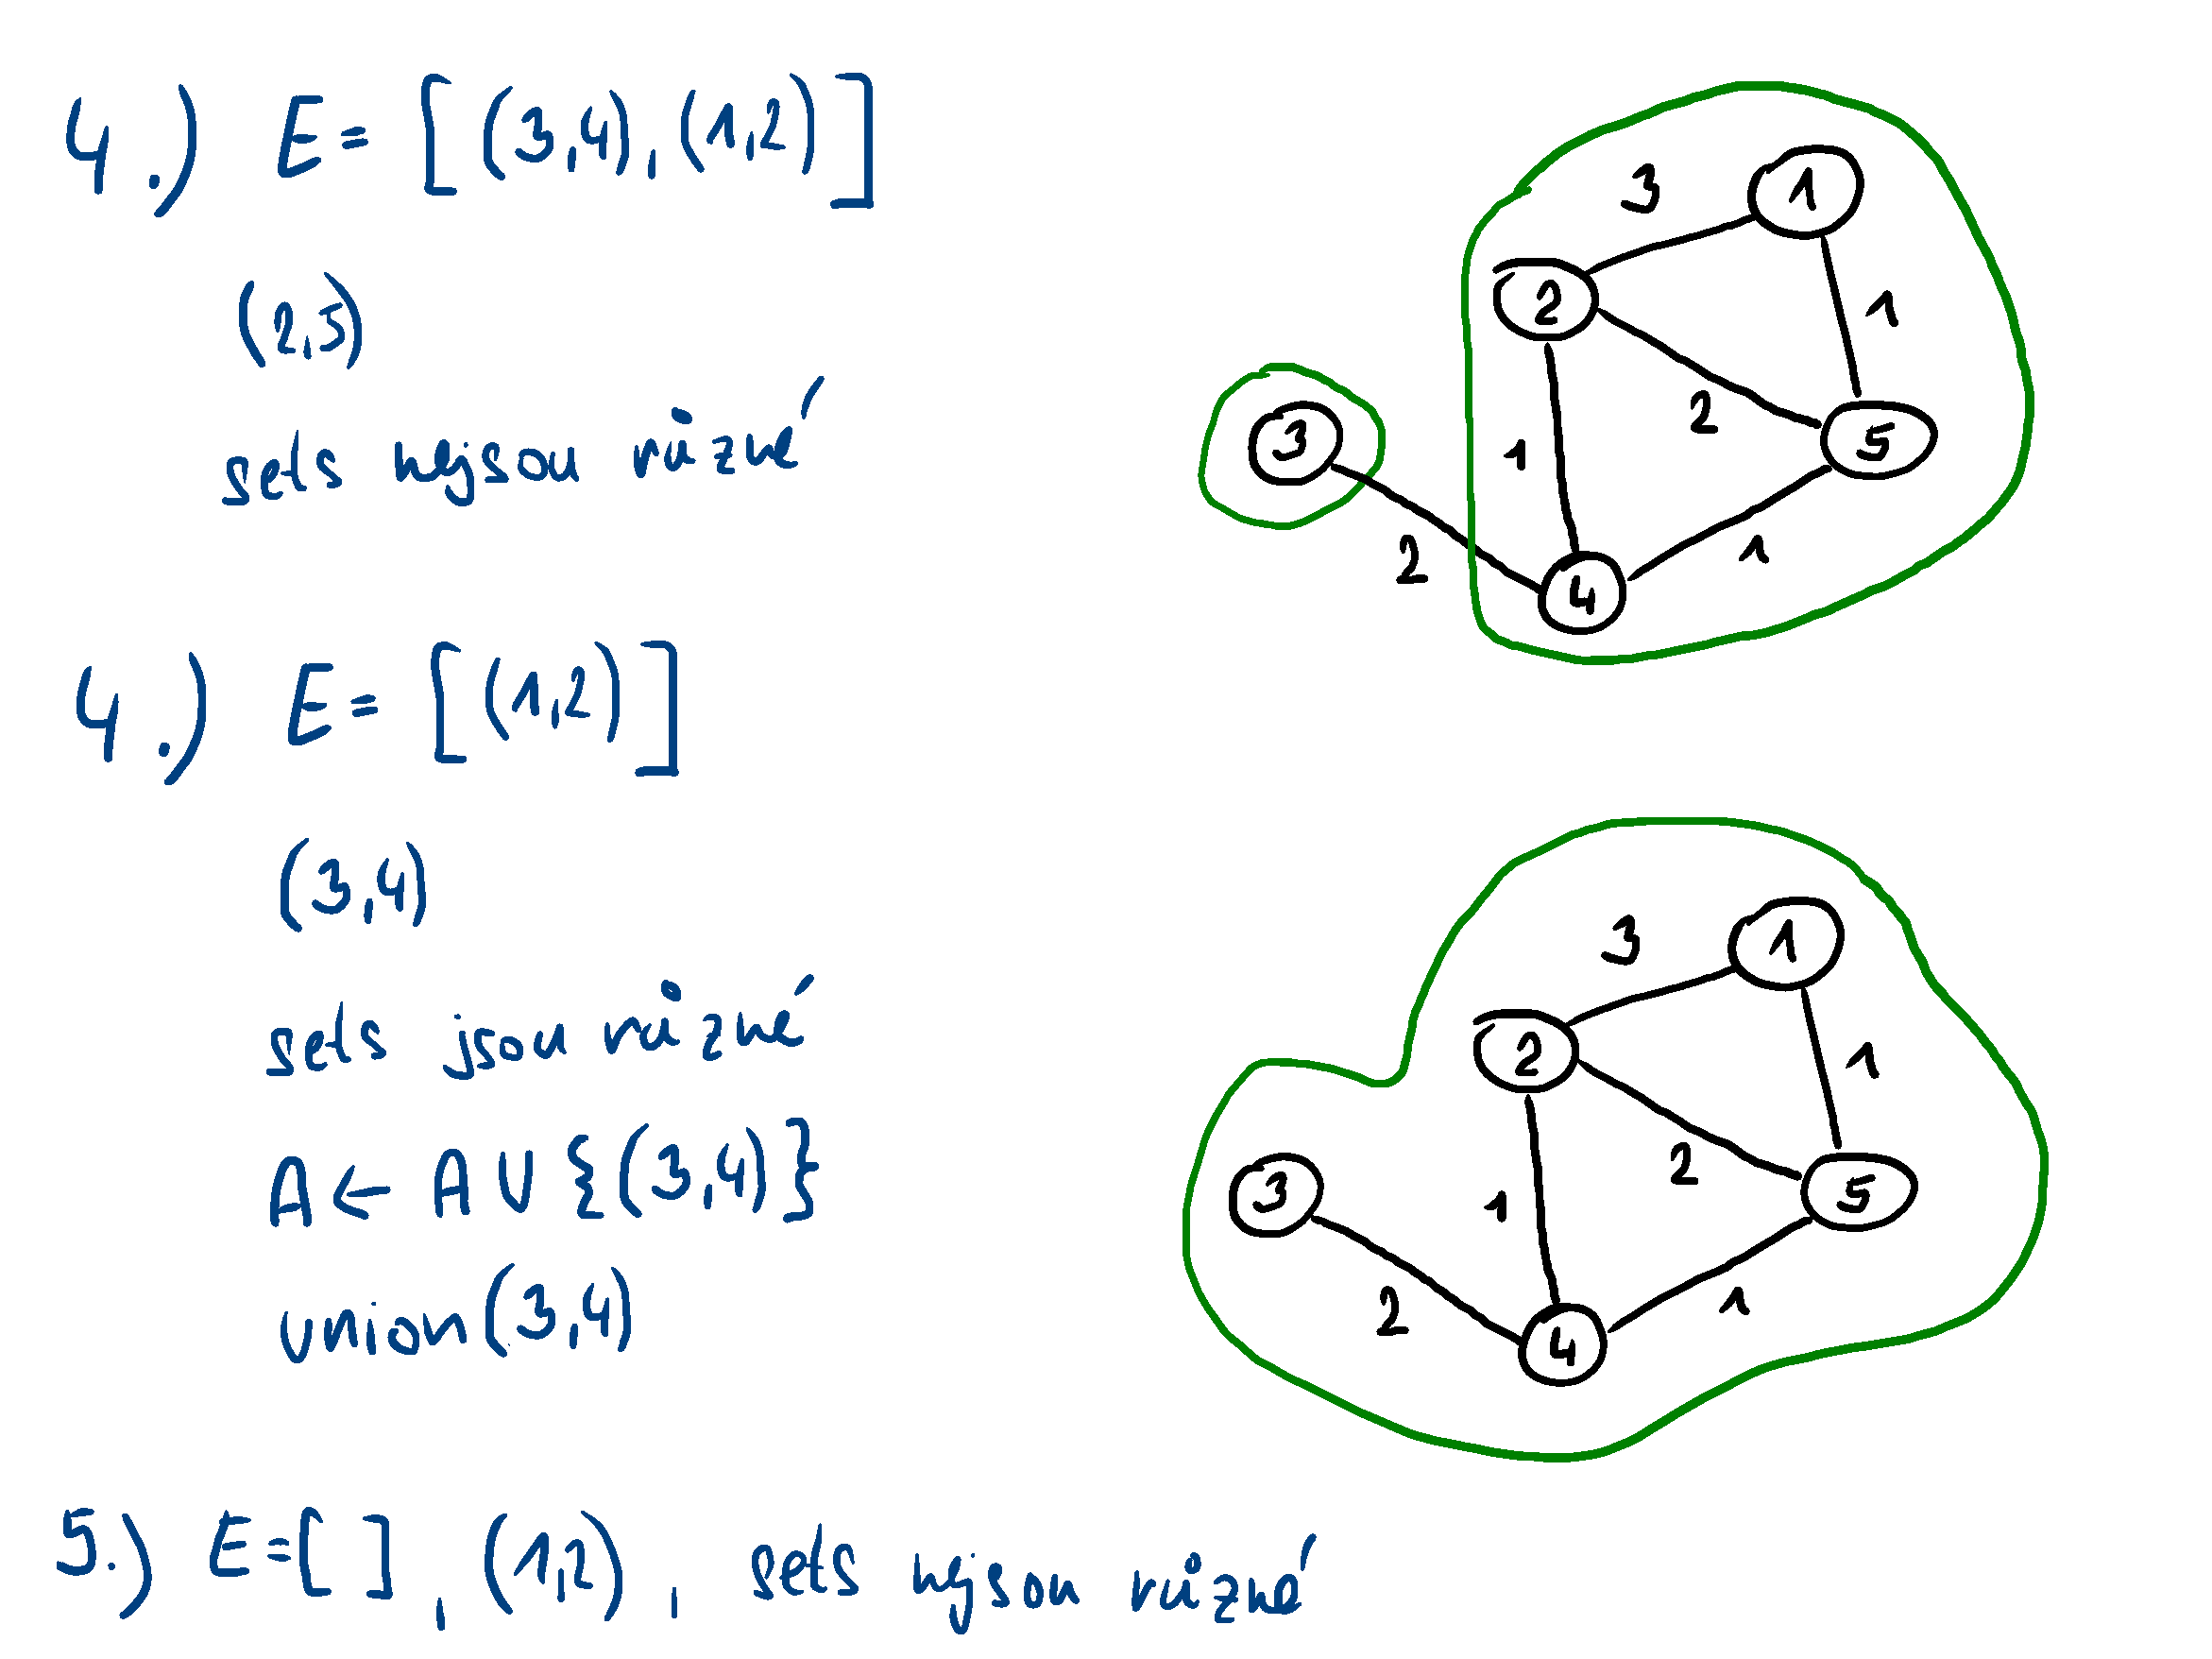
\includegraphics[width=0.9\linewidth]{45/03-minimalni-kostry-13.pdf}
    \caption{Příklad, část 3.}
\end{figure}

%%%%%%%%%%%%%%%%%%%%%%%%%%%%%%%%%%%%%%%%%%%%%%%%%%%%%%%%%%%%%%%%%%%%%%%%%%%%%%%%

\section{Primův-Jarníkův algoritmus}

Primův algoritmus buduje tzv. $A$ strom. Má zadaný určitý uzel, ze kterého hledá nejbližší další uzel, který by připojil. A pak další a další.

\bigskip\noindent\begin{minipage}{\linewidth}
\begin{lstlisting}[language=Python, caption={Primův algoritmus.}]
def prim_mst(G, r):
    # G je graf
    # r je vychozi uzel

    for u in G.V:
        key[u] = INF # pole cen prechodu, kolik stoji prechod do vrcholu na indexu
        pi[u] = NULL # pole predchudcu, kdo je predchudce vrcholu na indexu

    key[r] = 0
    Q = Queue(G.V) # prioritni fronta uzlu

    while not Q.empty():
        u = Q.extract_min(key) # vrati prvek z Q s nejmensi hodnotou v key

        # pro vsechny sousedy uzlu u (Adj je seznam sousedu)
        for v in Adj[u]:
            # pokud je levnejsi cesta a jeste to neni prozkoumany uzel
            if v in Q and w(u, v) < key(v):
                pi[v] = u
                key[v] = w(u, v)
                Q.decrease_key(key) # aktualizace prioritni fronty

    return pi
\end{lstlisting}
\end{minipage}

\subsection{Složitost}

\begin{itemize}
    \item Řádky 4-12 -- $O(n)$ za použití binární haldy ($n$ je počet uzlů).
    \item Řádky 14-15 -- While cyklus na řádku 14 se provede n-krát a protože \textit{extract\_min} stojí $O(\log(n))$, tak je celková složitost $O(n \cdot \log(n))$.
    \item Řádek 17 -- For cyklus se provede $O(m)$ krát, protože dálka všech seznamů sousedů je dohromady $2m$ ($m$ je počet hran).
    \item Řádek 19-21 -- $O(1)$.
    \item Řádek 23 -- stojí $O(\log(n))$, kvůli provedení operace $decrease\_key$ ve frontě $Q$.
    \item Jelikož $m > n$, tak celkem $O(n \cdot \log(n) + m \cdot \log(n)) = O(m \cdot \log(n))$.
\end{itemize}

\subsection{Příklad}

\begin{figure}[H]
    \centering
    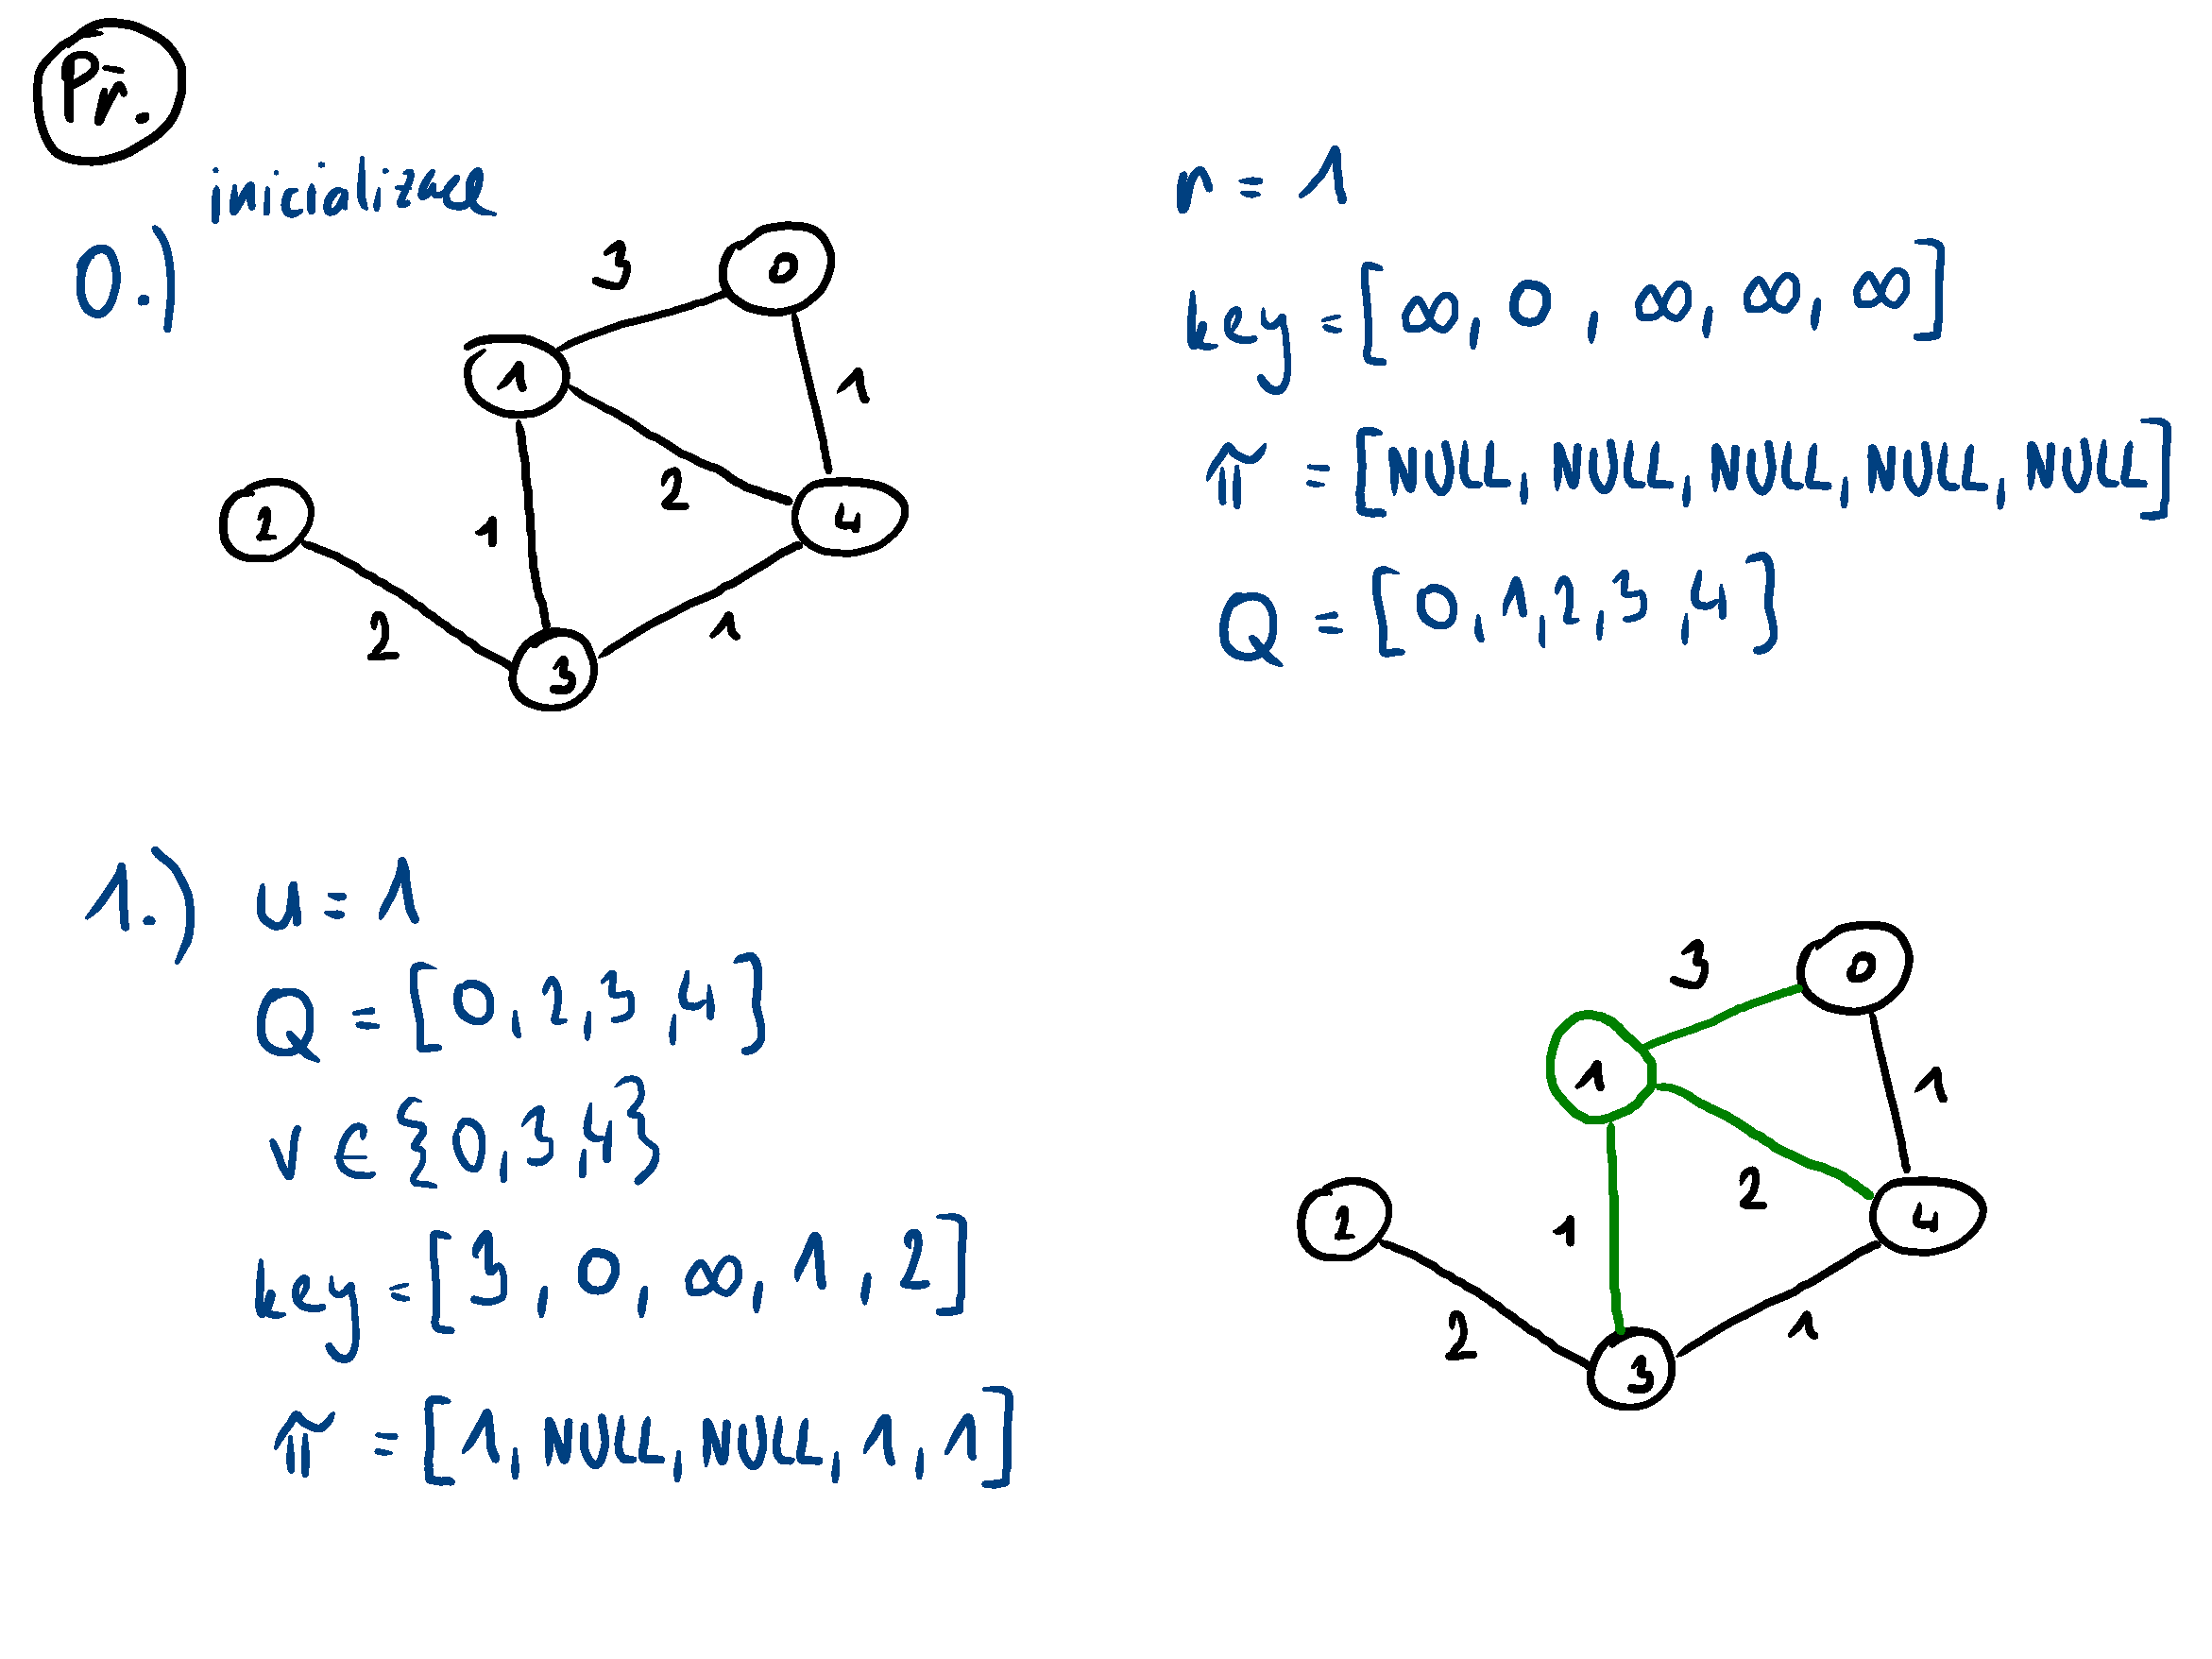
\includegraphics[width=0.9\linewidth]{45/03-minimalni-kostry-16.pdf}
    \caption{Příklad, část 1.}
\end{figure}

\begin{figure}[H]
    \centering
    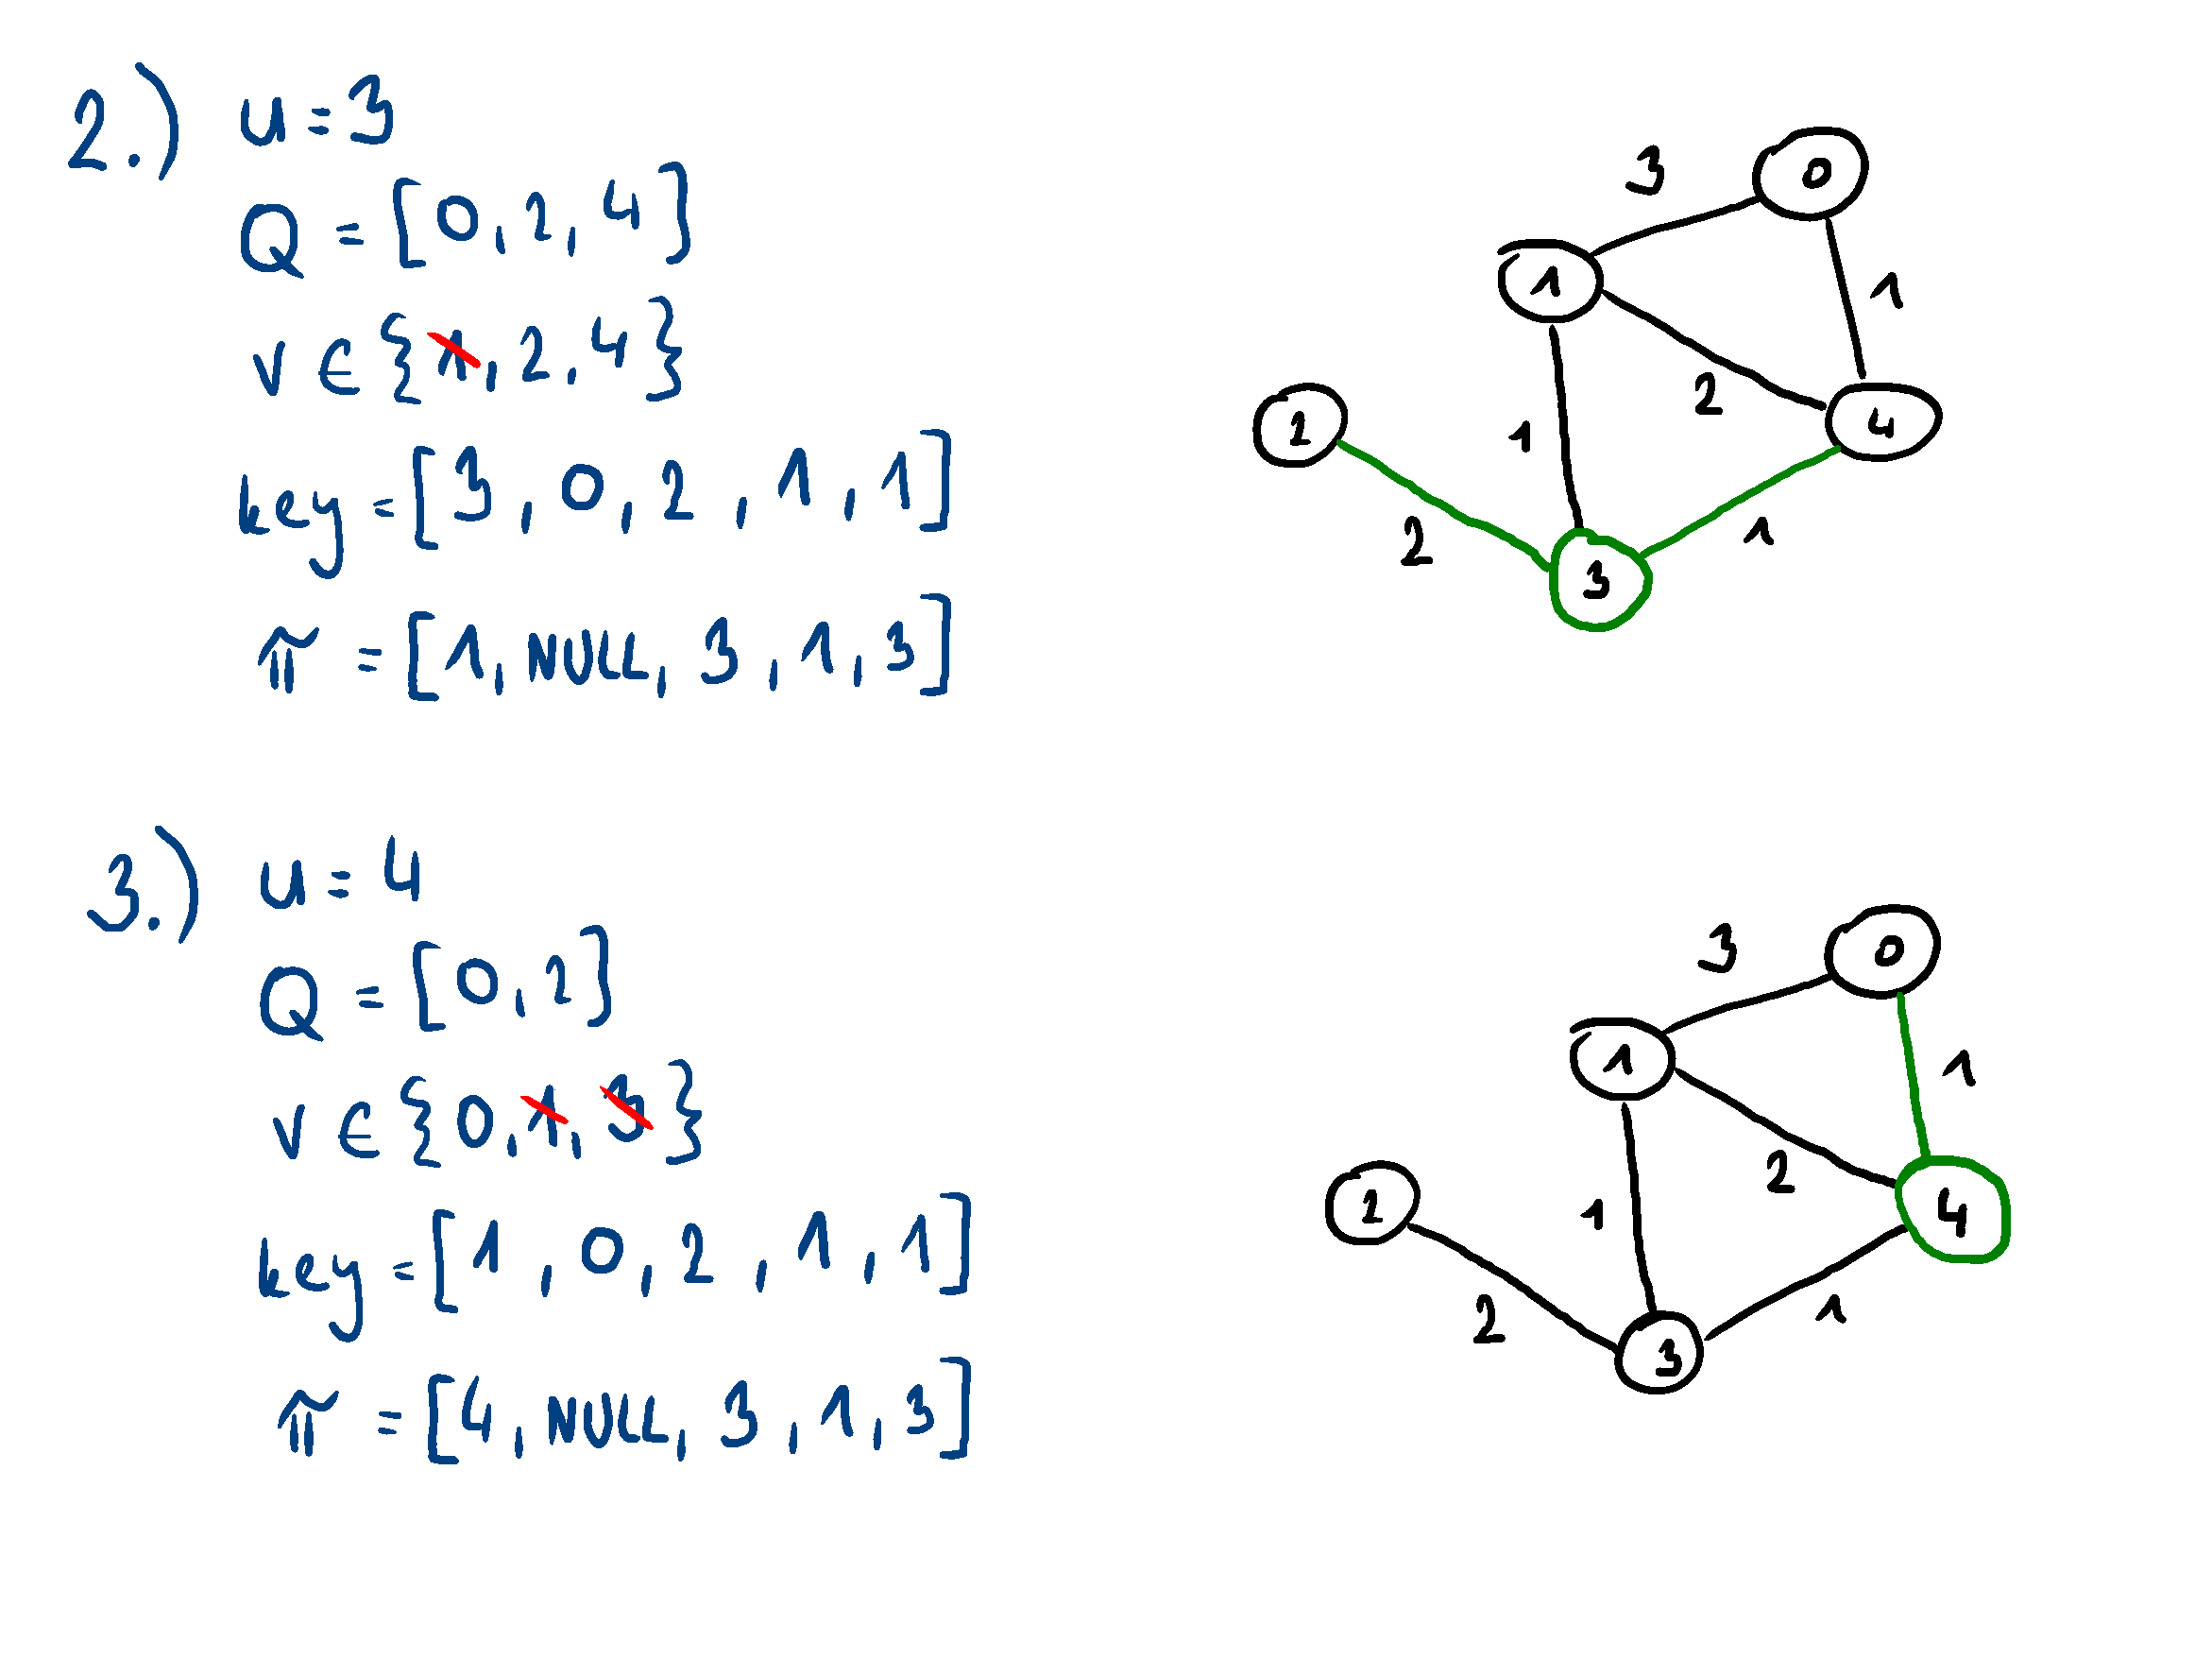
\includegraphics[width=0.9\linewidth]{45/03-minimalni-kostry-17.pdf}
    \caption{Příklad, část 2.}
\end{figure}

\begin{figure}[H]
    \centering
    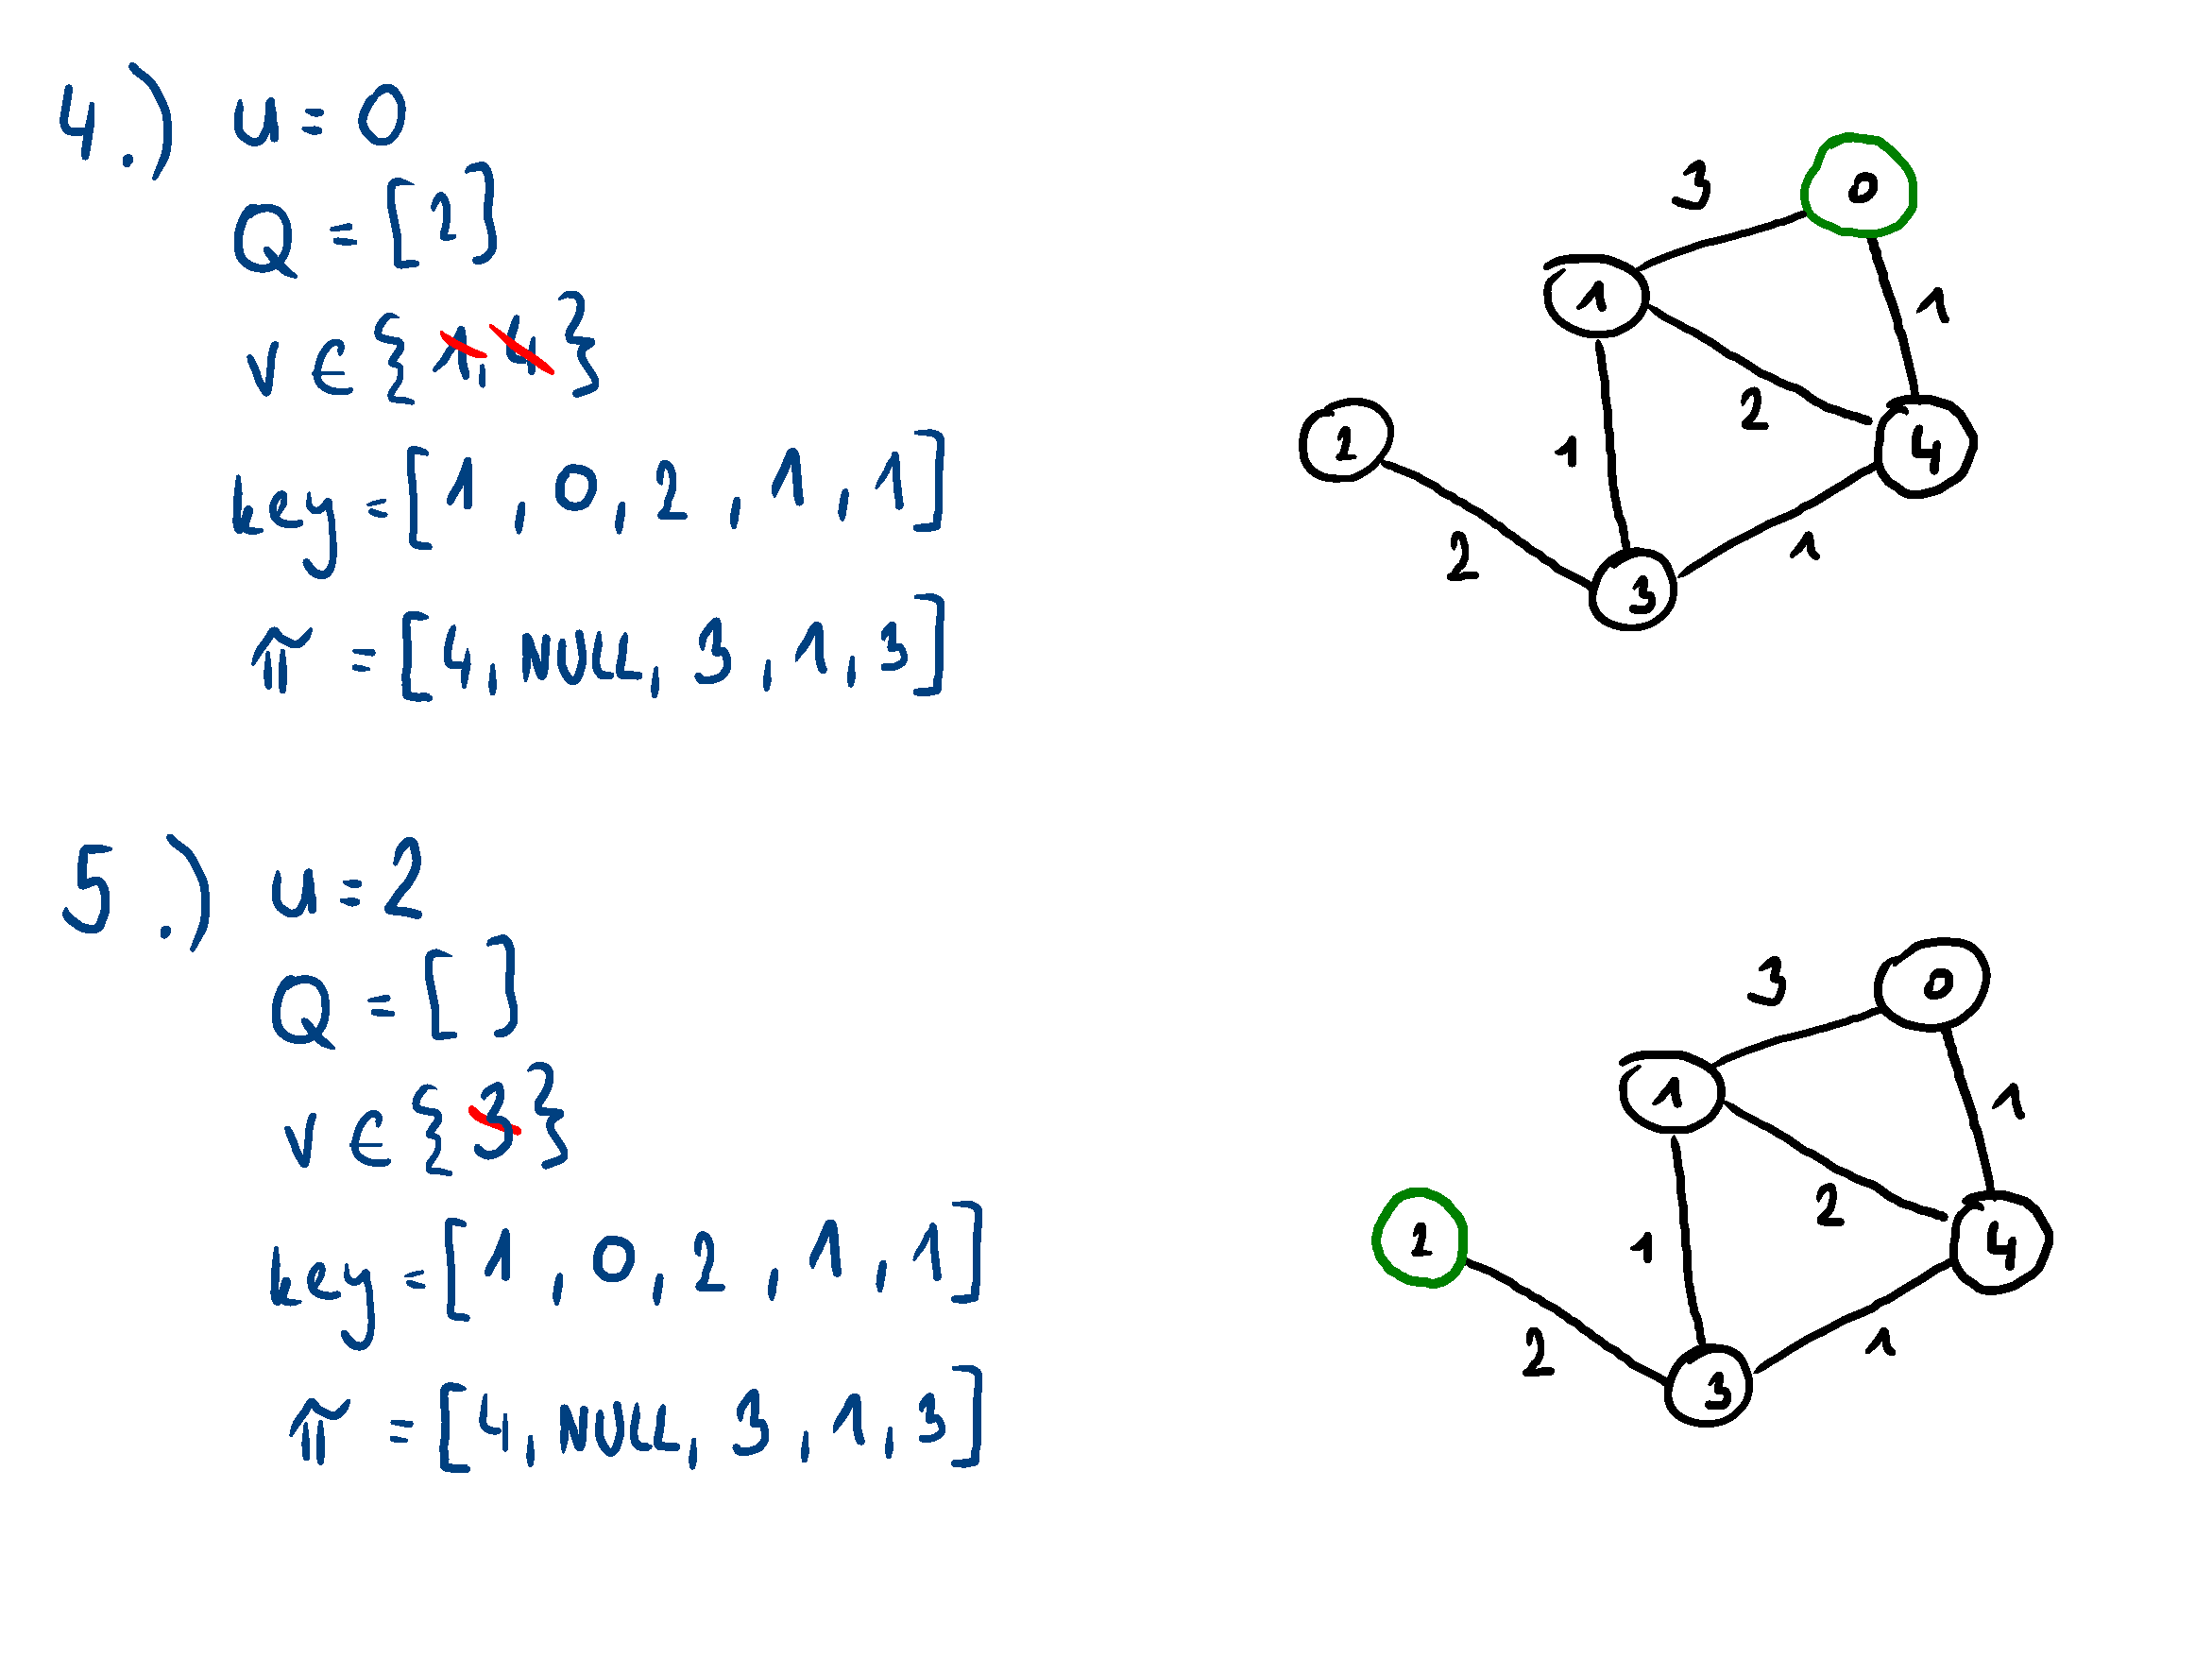
\includegraphics[width=0.9\linewidth]{45/03-minimalni-kostry-18.pdf}
    \caption{Příklad, část 3.}
\end{figure}

\begin{figure}[H]
    \centering
    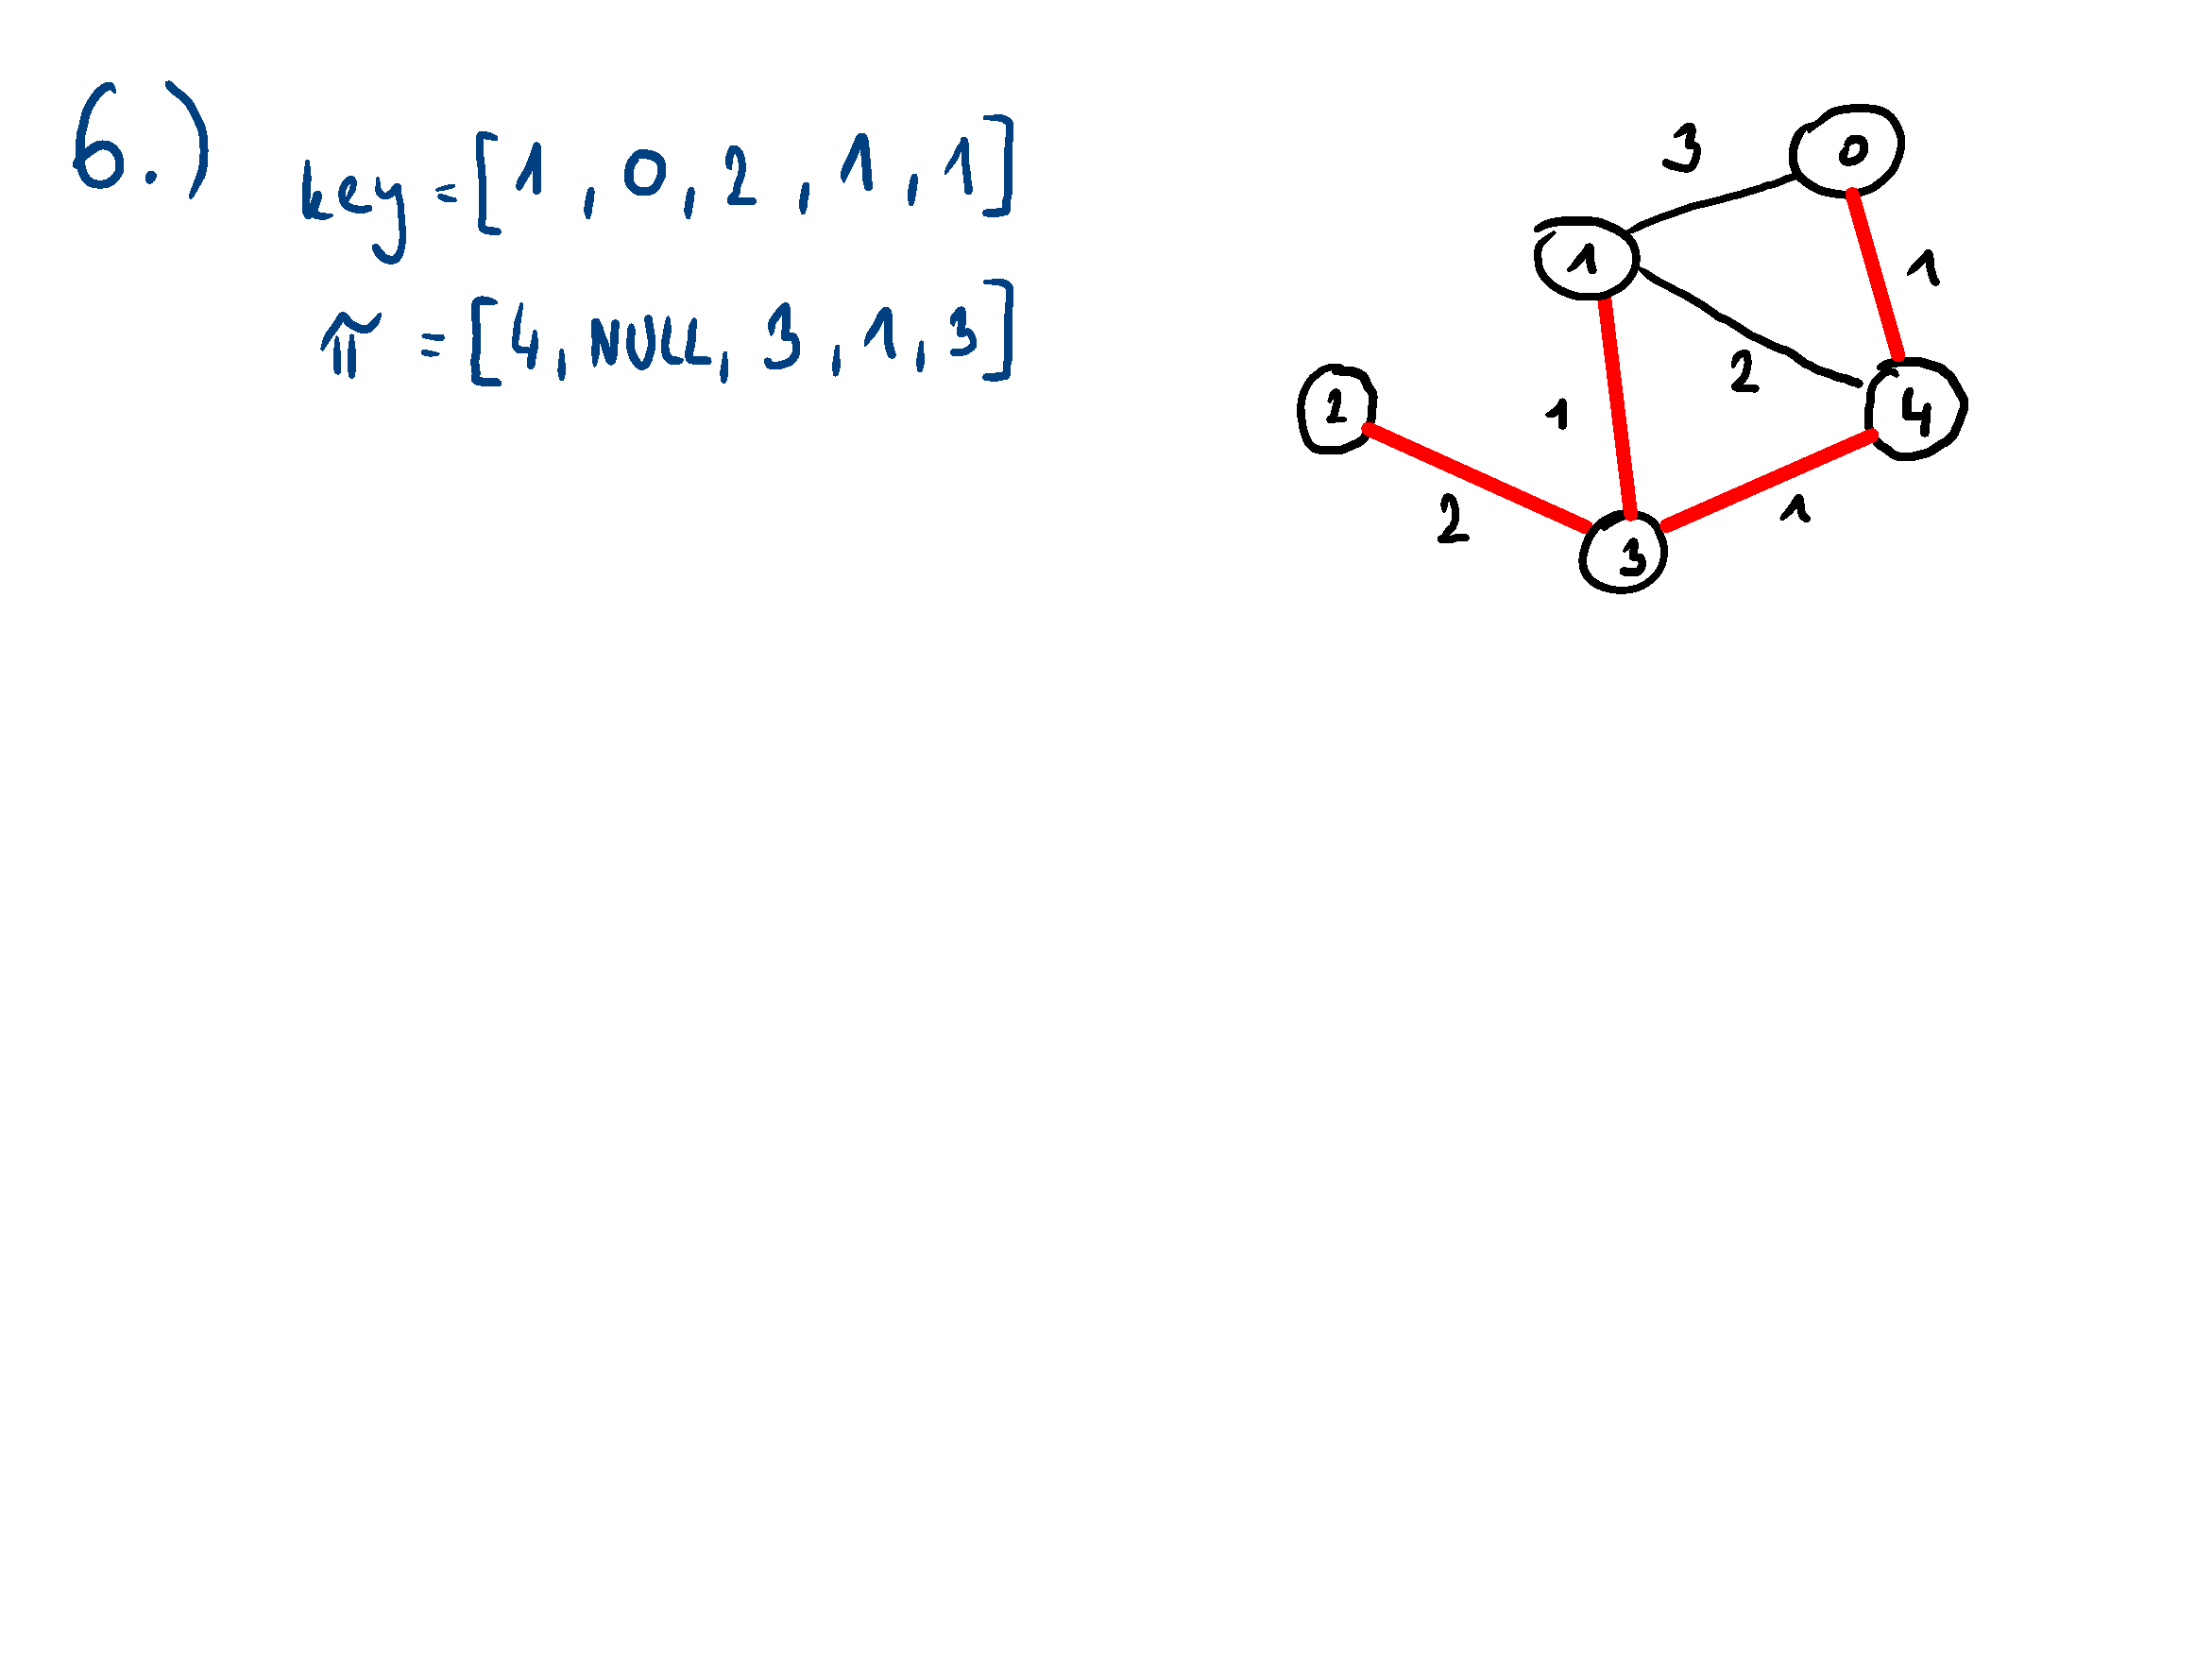
\includegraphics[width=0.9\linewidth]{45/03-minimalni-kostry-19.pdf}
    \caption{Příklad, část 4.}
\end{figure}

\newpage

% VUT FIT MITAI
% MSZ 2021/2022
% Author: Vladimir Dusek
% Login: xdusek27

%%%%%%%%%%%%%%%%%%%%%%%%%%%%%%%%%%%%%%%%%%%%%%%%%%%%%%%%%%%%%%%%%%%%%%%%%%%%%%%%

\chapter{Hledání nejkratších cest ze zdrojového uzlu do všech ostatních uzlů grafu (Bellman-Fordův algoritmus, Dijkstrův algoritmus).}

%%%%%%%%%%%%%%%%%%%%%%%%%%%%%%%%%%%%%%%%%%%%%%%%%%%%%%%%%%%%%%%%%%%%%%%%%%%%%%%%

\section{Metadata}

\begin{itemize}
    \item Předmět: Grafové algoritmy (GAL)
    \item Přednáška:
    \begin{itemize}
        \item 7) Nejkratší cesty z jednoho vrcholu, Bellman-Fordův algoritmus, nejkratší cesta z jednoho vrcholu v orientovaných acyklických grafech.
        \item 8) Dijkstrův algoritmus. Nejkratší cesty ze všech vrcholů.
    \end{itemize}
    \item Záznam:
    \begin{itemize}
        \item 2020-11-05
    \end{itemize}
\end{itemize}

%%%%%%%%%%%%%%%%%%%%%%%%%%%%%%%%%%%%%%%%%%%%%%%%%%%%%%%%%%%%%%%%%%%%%%%%%%%%%%%%

\section{Úvod a kontext}

\textit{Viz. \uv{Úvod a kontext} v předchozí otázce.}

\paragraph*{Cena cesty} Nechť $G = (V, E)$ je ohodnocený graf s váhovou funkcí $w: E \mapsto \mathbb{R}$. Cena cesty $p = \langle v_o, v_1, \dots, v_k \rangle$ je suma $$
w(p) = \sum_{i=0}^k w(v_i, v_{i+1})
$$.

\paragraph*{Cena nejkratší cesty} Cena nejkratší cesty z $u$ do $v$ je $$
\delta(u, v) = \begin{cases}
    min( \{ w(p) : u \xRightarrow{\text{p}} v \} ) \\
    \infty ~ \text{pokud cesta neexistuje}
\end{cases}
$$.

\paragraph*{Nejkratší cesta} Nejkratší cesta z $u$ do $v$ je pak libovolná cesta $p$ taková, že $w(p) = \delta(u, v)$.

\paragraph*{Cena cesty se záporným cyklem} Pokud na cestě z $u$ do $v$ existuje záporný cyklus (cyklus jehož celková cena je záporná), pak $\delta(u, v) = - \infty$.

\paragraph*{Záporné ohodnocení hran} Pokud na cestě z $u$ do $v$ neexistuje záporný cyklus, tak algoritmy pracují dobře i se záporným ohodnocením hran.

\paragraph*{Reprezentace cesty} Cestu reprezentujeme pomocí pole předchůdců $\pi$.

\paragraph*{Hledání nejkratších cest ze všech uzlů do jednoho} Tento problém lze řešit stejnými algoritmy. Graf se transponuje, provede se algoritmus pro problém \uv{hledání nejkratších cest ze jednoho uzlu do všech ostatních uzlů} a poté se transponuje zpět.

%%%%%%%%%%%%%%%%%%%%%%%%%%%%%%%%%%%%%%%%%%%%%%%%%%%%%%%%%%%%%%%%%%%%%%%%%%%%%%%%

\section{Pomocné funkce}

\noindent\begin{minipage}{\linewidth}
\begin{lstlisting}[language=Python, caption={Pomocná inicializační funkce.}]
def initialize_single_source(G, s):
    # G je graf
    # s je vychozi uzel
    for v in G.V:
        d[v] = INF  # d je pole vzdalenosti
        pi[v] = NULL  # pi je pole predchudcu
    d[s] = 0
\end{lstlisting}
\end{minipage}

\noindent\begin{minipage}{\linewidth}
\begin{lstlisting}[language=Python, caption={Pomocná funkce \textit{relax}.}]
def relax(u, v, w):
    # u a v jsou uzly grafu
    # w je vahova funkce
    if d[v] > d[u] + w(u, v):
        d[v] = d[u] + w(u, v)
        pi[v] = u
\end{lstlisting}
\end{minipage}

\begin{figure}[H]
    \centering
    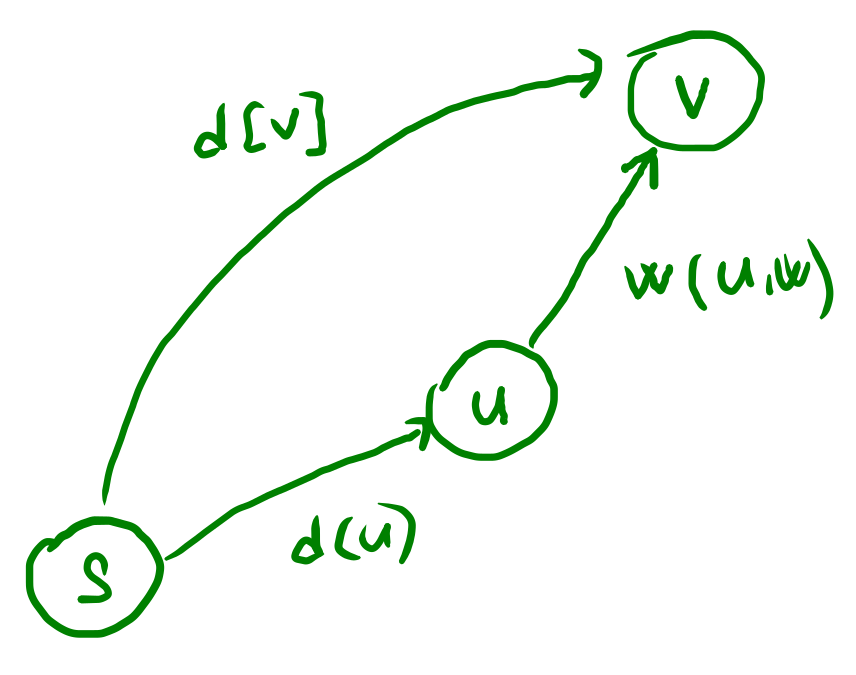
\includegraphics[width=0.4\linewidth]{46/relax.png}
    \caption{Ukázka činnosti funkce \textit{relax}.}
\end{figure}

%%%%%%%%%%%%%%%%%%%%%%%%%%%%%%%%%%%%%%%%%%%%%%%%%%%%%%%%%%%%%%%%%%%%%%%%%%%%%%%%

\section{Bellman-Fordův algoritmus}

Slouží pro řešení v obecných grafech (mohou obsahovat cykly a záporné hrany).

\bigskip\noindent\begin{minipage}{\linewidth}
\begin{lstlisting}[language=Python, caption={Algoritmus Bellman-Ford.}]
def bellman_ford(G, s, w):
    # G je graf
    # s je vychozi uzel
    # w je vahova funkce

    # faze inicializace
    initialize_single_source(G, s)
    n = len(G.V) # pocet uzlu

    # faze relaxace: provedeni n * (n-1) relaxaci
    for _ in range(0, n-1):
        for u, v in G.E:
            relax(u, v, w)

    # faze detekce zaporneho cyklu
    for u, v in G.E:
        if d[u] > d[v] + w(u, v):
            return NULL

    return d, pi
\end{lstlisting}
\end{minipage}

%%%%%%%%%%%%%%%%%%%%%%%%%%%%%%%%%%%%%%%%%%%%%%%%%%%%%%%%%%%%%%%%%%%%%%%%%%%%%%%%

\section{Dijkstrův algoritmus}

Slouží pro řešení v acyklických grafech bez záporných hran. Pro takto omezený problém existují rychlejší algoritmy než pro problém v obecných grafech.

\bigskip\noindent\begin{minipage}{\linewidth}
\begin{lstlisting}[language=Python, caption={Algoritmus Dijkstra.}]
def dijkstra(G, s, w):
    # G je graf
    # s je vychozi uzel
    # w je vahova funkce

    # faze inicializace
    initialize_single_source(G, s)
    Q = Queue(G.V) # prioritni fronta uzlu

    # faze relaxace
    while not Q.empty():
        u = Q.extract_min(d) # vrati prvek z Q s nejmensi hodnotou v d

        # pro vsechny sousedy uzlu u (Adj je seznam sousedu)
        for v in Adj[u]:
            relax(u, v, w)

    return d, pi
\end{lstlisting}
\end{minipage}

\newpage

% VUT FIT MITAI
% MSZ 2021/2022
% Author: Vladimir Dusek
% Login: xdusek27

%%%%%%%%%%%%%%%%%%%%%%%%%%%%%%%%%%%%%%%%%%%%%%%%%%%%%%%%%%%%%%%%%%%%%%%%%%%%%%%%

\chapter{Klasifikace algoritmů volby koordinátora, algoritmus Bully a jeho složitost.}

%%%%%%%%%%%%%%%%%%%%%%%%%%%%%%%%%%%%%%%%%%%%%%%%%%%%%%%%%%%%%%%%%%%%%%%%%%%%%%%%

\section{Metadata}

\begin{itemize}
    \item Předmět: Grafové algoritmy (GAL)
    \item Přednáška:
    \begin{itemize}
        \item 7) Synchronizace
    \end{itemize}
    \item Záznam:
    \begin{itemize}
        \item 2020-11-02
    \end{itemize}
\end{itemize}

%%%%%%%%%%%%%%%%%%%%%%%%%%%%%%%%%%%%%%%%%%%%%%%%%%%%%%%%%%%%%%%%%%%%%%%%%%%%%%%%

\section{Úvod a kontext}

\begin{itemize}
    \item Mějme množinu procesů v rámci distribuovaného systému. Řešíme problém  nalezení shody na nějaké věci (synchronizační problém). Problém můžeme rozdělit na dvě situace:
    \begin{itemize}
        \item \textbf{Problém volby koordinátora} -- Výběr jednoho z procesů, který bude vedoucím procesem (koordinátor). Tento proces pak může vykonat určitou činnost nebo může sloužit ostatním procesům k realizaci  význačné role v systému.
        \item \textbf{Problém vzájemného vyloučení} -- Předpokládejme, že konkrétní zdroj může v daném okamžiku používat pouze jeden proces. Tento problém se běžně vyskytuje ve víceprocesorových systémech, ale také v distribuovaných systémech.
    \end{itemize}
    \item Synchronizační problémy lze v rámci operačních systémů nebo multiprocesorových systémů řešit pomocí provádění atomických operací, sdílené paměti apod. (je pro ně podpora v rámci operačního systému nebo hardwaru). V distribuovaných systémech nic takového není z principu možné a proto se synchronizační problémy řeší pomocí zasílání zprav, resp. algoritmicky.
\end{itemize}

%%%%%%%%%%%%%%%%%%%%%%%%%%%%%%%%%%%%%%%%%%%%%%%%%%%%%%%%%%%%%%%%%%%%%%%%%%%%%%%%

\section{Problém volby koordinátora}

\begin{itemize}
    \item Předpokládáme:
    \begin{itemize}
        \item Každý proces má unikátní ID.
        \item Procesy neznají stav (běžící, neběžící) dalších procesů.
        \item Každý proces zná ID dalších procesů (záleží na topologii).
    \end{itemize}
    \item Cíl:
    \begin{itemize}
        \item Dosáhnutí shody mezi všemi procesy na procesu, který je koordinátor.
        \item Kritérium výběru koordinátora může být různé. Např. na základě proces ID (proces s největším ID se stane koordinátorem).
    \end{itemize}
\end{itemize}

%%%%%%%%%%%%%%%%%%%%%%%%%%%%%%%%%%%%%%%%%%%%%%%%%%%%%%%%%%%%%%%%%%%%%%%%%%%%%%%%

\section{Bully algoritmus}

Pro topologii každý s každým -- každý proces může komunikovat s každým dalším procesem. Používá tři druhy zpráv: ELECTION, OK, COORDINATOR.

\subsection*{Postup}

\begin{itemize}
    \item Proces P, který má podezření, že chybí koordinátor, může zahájit volby.
    \begin{enumerate}
        \item Proces P odešle zprávu ELECTION všem procesům s větším ID.
        \item Pokud nikdo neodpoví, P vyhrává volby a stává se koordinátorem.
        \item Pokud některý z procesů s větším ID odpoví (zpráva OK), tak přebírá řízení a práce P je ukončena.
        \item Pokud P obdrží zprávu ELECTION od procesů s menším ID, pošle jim odpověď OK na zablokování procesů.
    \end{enumerate}
    \item Nakonec zůstane pouze P (nový koordinátor), který o tom informuje ostatní zasláním zprávy COORDINATOR.
    \item Pokud se proces probudí nebo je restartován, první akcí je vyvolání voleb.
\end{itemize}

\subsection*{Složitost}

Složitost z hlediska počtu zpráv.

\bigskip\noindent Nejhorší případ (iniciátor s nejmenším ID):

\begin{itemize}
    \item $(n-1)$ iterací
    \item $2(n-1)$ zpráv ELECTION a OK pro každou iteraci
    \item $(n-1)$ zpráv COORDINATOR
    \item Celkem: $(n-1) \times 2(n-1) + (n-1) \approx n^2$
\end{itemize}

\noindent Nejlepší případ (iniciátor s největším ID):

\begin{itemize}
    \item $(n-1)$ zpráv COORDINATOR
    \item Celkem: $(n-1)$
\end{itemize}

\subsection*{Příklad}

\begin{figure}[H]
    \centering
    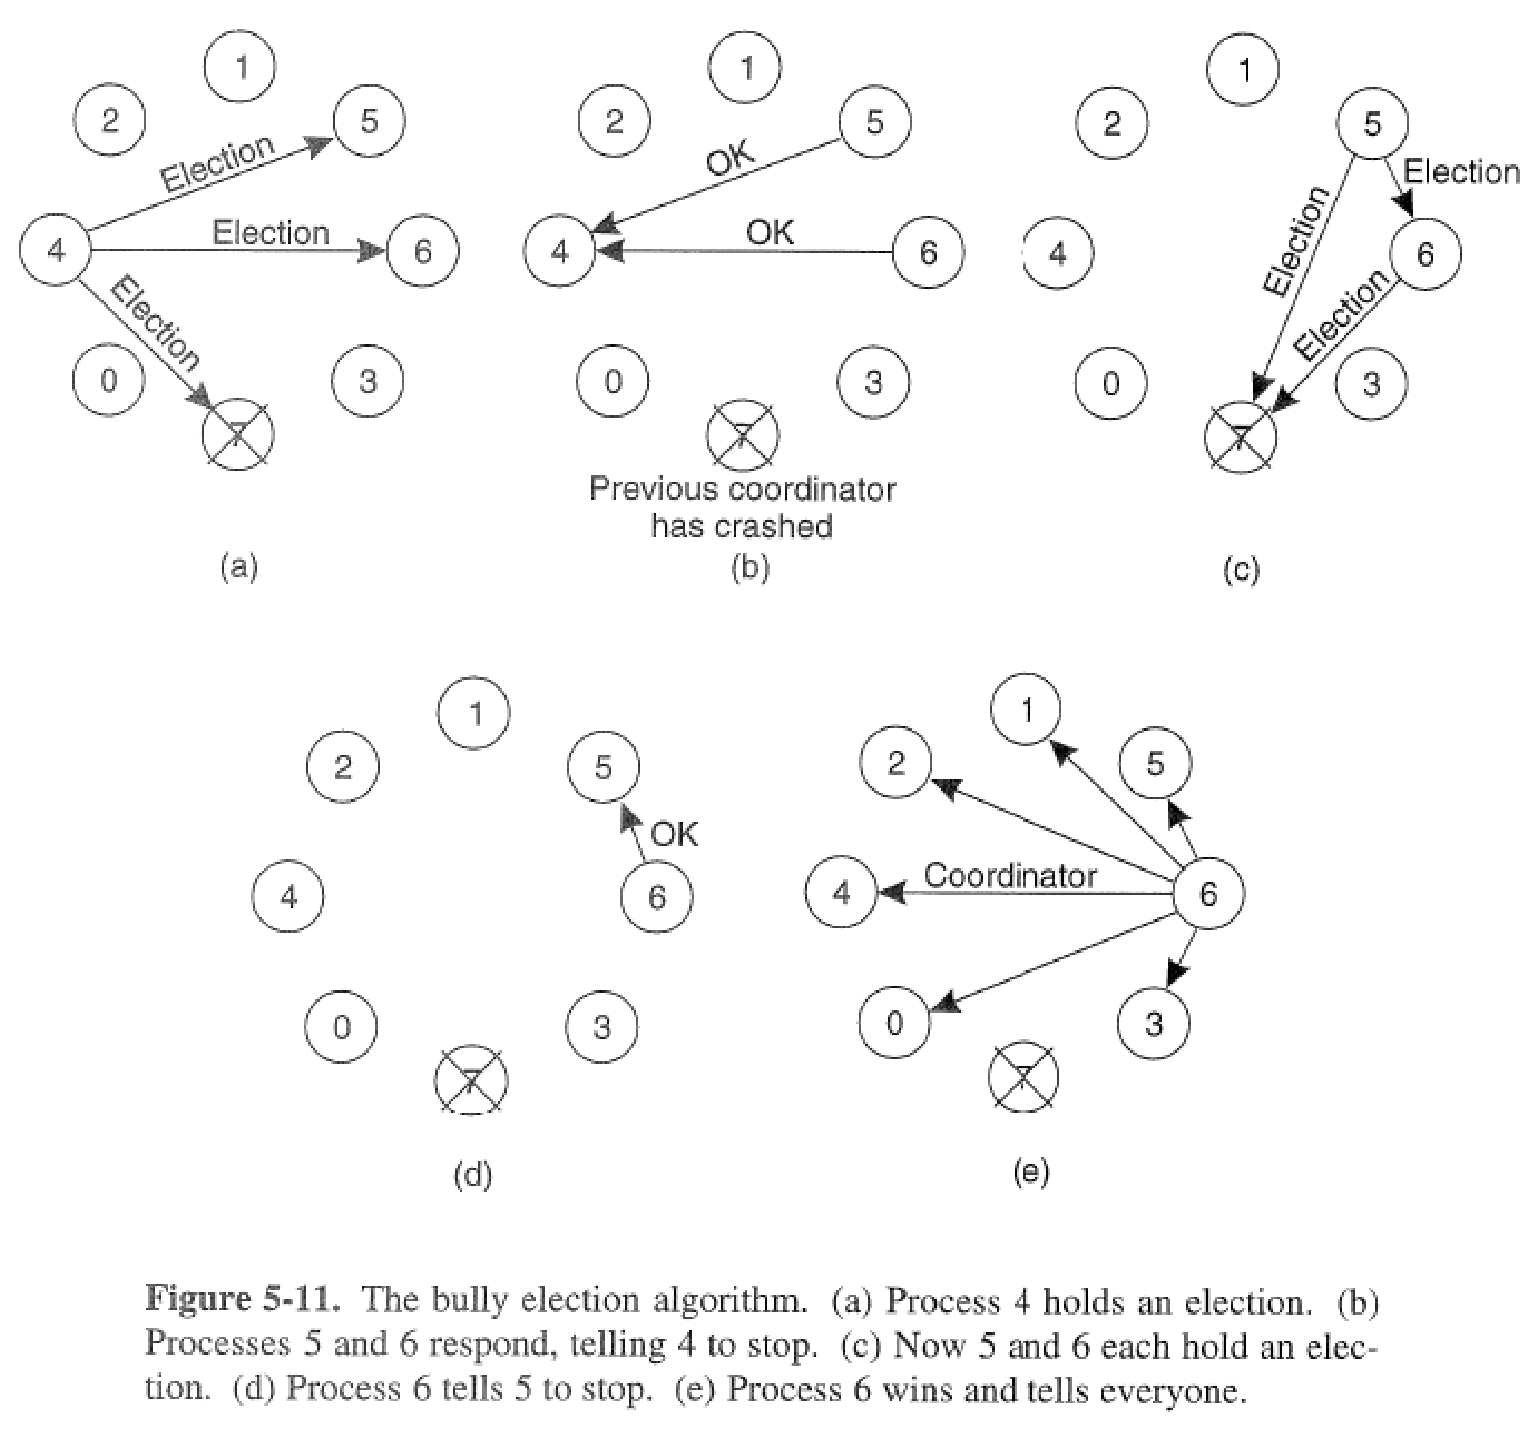
\includegraphics[width=1\linewidth]{47/example_bully.pdf}
    \caption{Příklad činnosti Bully algoritmu.}
\end{figure}

%%%%%%%%%%%%%%%%%%%%%%%%%%%%%%%%%%%%%%%%%%%%%%%%%%%%%%%%%%%%%%%%%%%%%%%%%%%%%%%%

\section{Ring Algoritmus}

Pro kruhovou topologii -- procesy jsou uspořádané do kruhu podle svého proces ID.
Každý proces musí vědět nejenom o svém následovníkovi, ale také o jeho následníkovi, který funguje jako \uv{záloha}, v případě že by se přímý následník stal nedostupný. Používá dva druhy zpráv: ELECTION, COORDINATOR.

\subsection*{Postup}

\begin{itemize}
    \item Proces P, který má podezření, že chybí koordinátor, může zahájit volby.
    \begin{enumerate}
        \item Zašle zprávu ELECTION obsahující jeho ID dalšímu procesu (pokud další proces nereaguje, proces P zašle stejnou zprávu dalšímu v kruhu).
        \item Každý člen topologie přijme zprávu ELECTION, přidá do ní své ID a přepošle zprávu dalšímu procesu.
    \end{enumerate}
    \item Když se zpráva vrátí k procesu P, je zpráva převedena na zprávu  COORDINATOR a poslána následujícímu procesu v topologii, aby bylo možné nahlásit:
    \begin{enumerate}
        \item Novým koordinátorem se stává proces s nejvyšším ID.
        \item Členové sítě jsou stále aktivní.
    \end{enumerate}
    \item Po síti může obíhat více zpráv zároveň.
\end{itemize}

\subsection*{Složitost}

Složitost z hlediska počtu zpráv.

\bigskip\noindent Vždy $2n \approx n$ zpráv. Jedno kolečko \uv{oběhne} zpráva ELECTION a druhé zpráva COORDINATOR.

\subsection*{Příklad}

\begin{figure}[H]
    \centering
    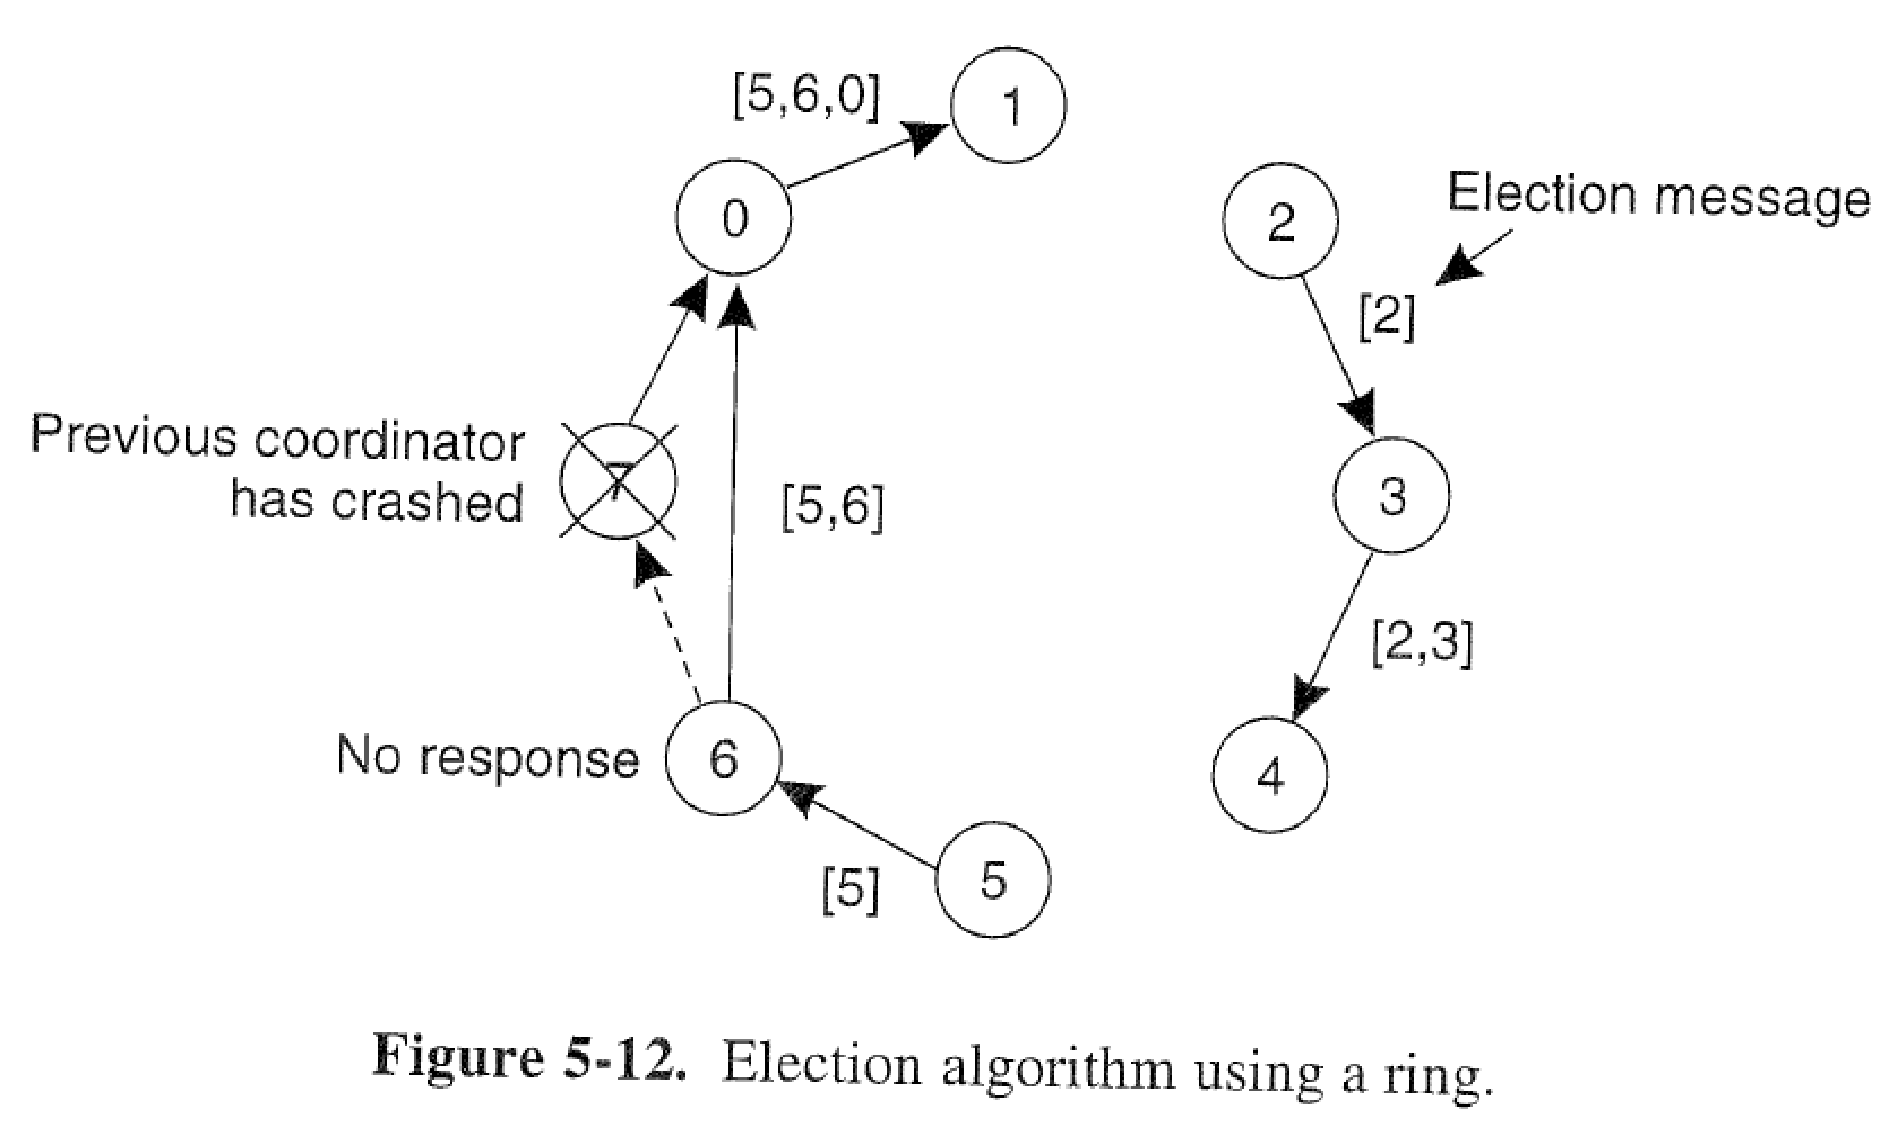
\includegraphics[width=1\linewidth]{47/example_ring.pdf}
    \caption{Příklad činnosti Ring algoritmu.}
\end{figure}

%%%%%%%%%%%%%%%%%%%%%%%%%%%%%%%%%%%%%%%%%%%%%%%%%%%%%%%%%%%%%%%%%%%%%%%%%%%%%%%%

\section{Algoritmus pro obecnou topologii}

Předpokládáme, že nemáme ani kruhovou topologii ani spojení každý s každým. Např.: peer-to-peer sítě, sensorové sítě, \dots

\subsection*{Postup}

\begin{itemize}
    \item V první iteraci se broadcastem posílá zpráva ELECTION.
    \item Každý uzel si uloží od kterého souseda dostal zprávu ELECTION jako první. Tím vzníká kostra grafu (\textit{spanning tree}).
    \item Uložený soused je poté využijí pro zpětnou komunikaci. To znamená, že další komunikace už probíhá přes strom, nikoliv přes broadcast. Tím je ušetřena některé komunikace.
\end{itemize}

\subsection*{Složitost}

Složitost z hlediska počtu zpráv.

\begin{itemize}
    \item Inicializační broadcast: počet hran grafu.
    \item Odpověď: počet hran kostry grafu.
    \item Result broadcast: počet hran kostry grafu.
\end{itemize}

\subsection*{Příklad}

\begin{figure}[H]
    \centering
    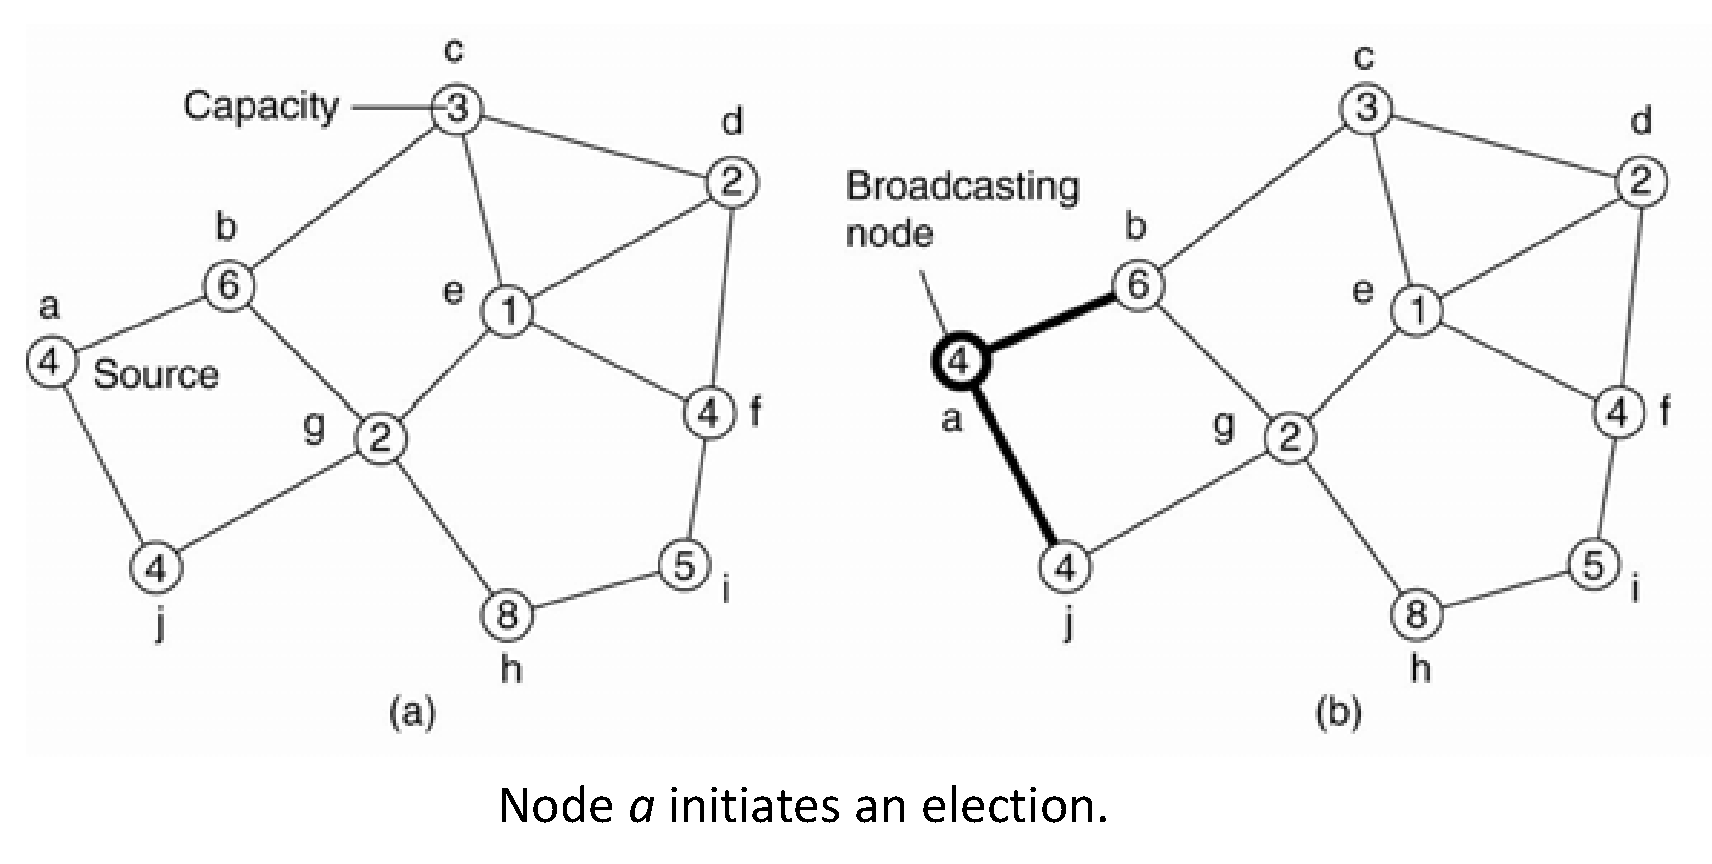
\includegraphics[width=1\linewidth]{47/example_general_topology_p1.pdf}
    \caption{Příklad činnosti algoritmu pro obecnou topologii, část 1.}
\end{figure}

\begin{figure}[H]
    \centering
    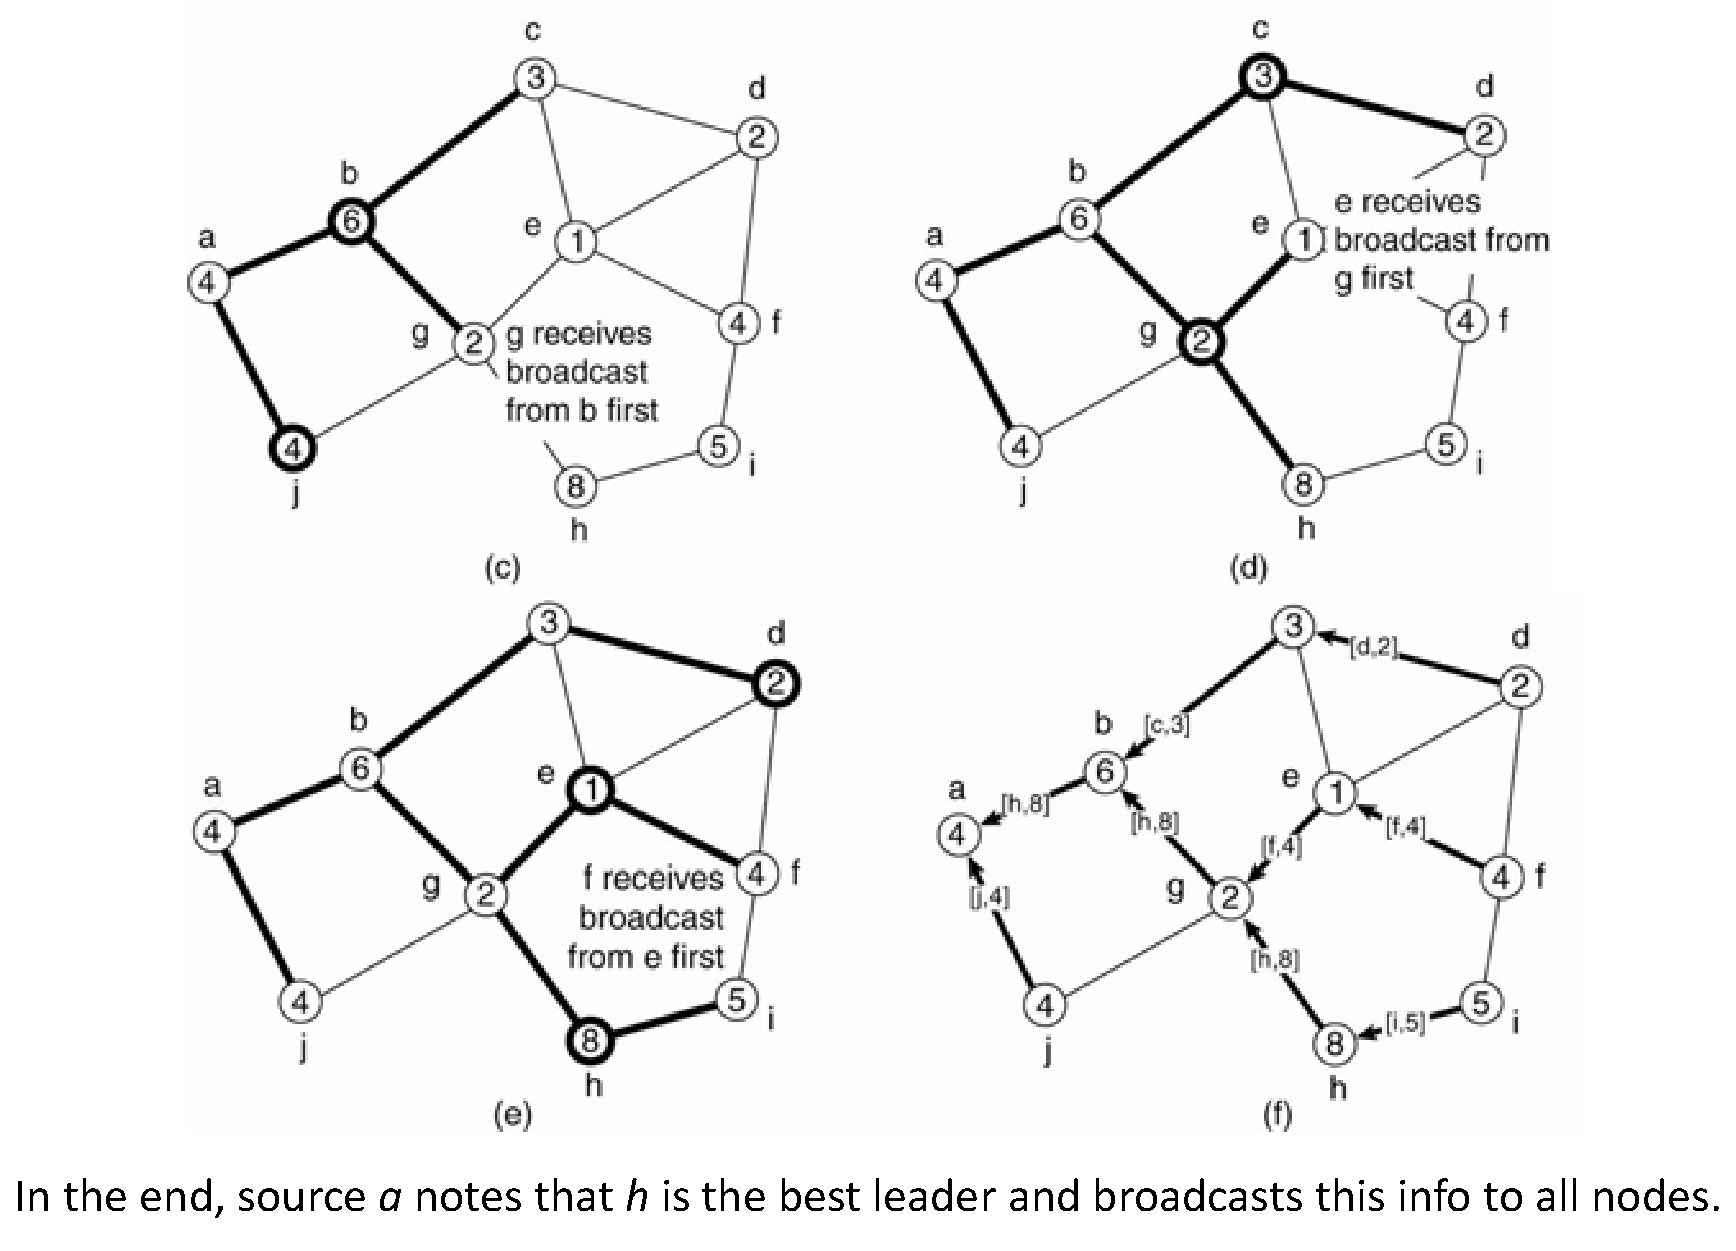
\includegraphics[width=1\linewidth]{47/example_general_topology_p2.pdf}
    \caption{Příklad činnosti algoritmu pro obecnou topologii, část 2.}
\end{figure}

\newpage

% VUT FIT MITAI
% MSZ 2021/2022
% Author: Vladimir Dusek
% Login: xdusek27

%%%%%%%%%%%%%%%%%%%%%%%%%%%%%%%%%%%%%%%%%%%%%%%%%%%%%%%%%%%%%%%%%%%%%%%%%%%%%%%%

\chapter{Podmínky konsistentního globálního stavu distribuovaného systému.}

\subsection*{Metadata}

\begin{itemize}
    \item Předmět: Prostředí distribuovaných aplikací (PDI)
    \item Přednáška:
    \begin{itemize}
        \item 4) Globální stav a snapshots
    \end{itemize}
    \item Záznam:
    \begin{itemize}
        \item 2020-10-12
    \end{itemize}
\end{itemize}

%%%%%%%%%%%%%%%%%%%%%%%%%%%%%%%%%%%%%%%%%%%%%%%%%%%%%%%%%%%%%%%%%%%%%%%%%%%%%%%%

\section{Úvod a kontext}

\paragraph*{Distribuovaný systém} Distribovaný systém je množina procesů $p_1, p_2, \dots, p_n$, které jsou propojeny komunikačními kanály. V systému neexistuje žádná globální paměť ani globální hodiny. Procesy spolu komunikují pouze zasíláním zpráv skrze komunikačními kanály.

\paragraph*{Komunikační kanál} Komunikační kanál mezi procesy $p_i$ a $p_j$ značíme $C_{ij}$.

\paragraph*{Událost} Rozlišujeme tři typy událostí: interní událost procesu, zaslání zprávy a přijetí zprávy.

\paragraph*{Zpráva} Zpráva $m_{ij}$ značí zprávu zaslanou procesem $p_i$ procesu $p_j$. $send(m_{ij})$ značí odeslání zprávy a $recv(m_{ij})$ přijetí.

\paragraph*{Stav procesu} Lokální stav procesu $p_i$ značíme $LS_i$. Lokální stav je definován jako sekvence všech událostí, o kterých proces $p_i$ ví. Nechť $e$ je libovolná událost, $e \in LS_i$ značí, že událost $e$ patří do lokálního stavu procesu $p_i$, $e \not\in LS_i$ značí, že událost $e$ nepatří do lokálního stavu procesu $p_i$.

\paragraph*{Stav komunikačního kanálu} Stav komunikačního kanálu $C_{ij}$ značíme $SC_{ij}$ a je definován množinou zpráv, které obsahuje. Pro kanál $C_{ij}$ můžeme definovat jeho stav na základě lokálních stavů procesů $LS_i$ a $LS_j$: $$
transit(LS_i, LS_j) = \{ m_{ij} \,|\, send(m_{ij}) \in LS_i \land rec(m_{ij}) \not\in LS_j \}
$$.

\section{Model komunikace}

\begin{itemize}
    \item FIFO -- Komukační kanál funguje jako fronta zpráv \textit{first in}, \textit{first out}. Kanál tedy zachovává pořadí zpráv sám o sobě.

    \item non-FIFO -- Komunikační kanál se chová jako datová struktura množina, do které odesílatel vkládá zprávy a příjemce je odebírá v náhodném pořadí.

    \item Causal ordering (kauzální uspořádání) -- Systém, který podporuje kauzální doručení zpráv splňuje následující vlastnost. Pro jakékoliv dvě zprávy $m_{ij}$ a $m_{kj}$ platí, pokud $send(m_{ij}) \rightarrow send(m_{kj})$, pak i $recv(m_{ij}) \rightarrow recv(m_{kj})$.
\end{itemize}

\section{Konzistentní globální stav}

\paragraph*{Globální stav} Globální stav distribuovaného systému je kolekce lokálních stavů procesů a komunikačních kanálů. $$
GS = \Big\{ \bigcup_{i} LS_i \,,\, \bigcup_{i, j} SC_{ij} \Big\}
$$.

\paragraph*{Časoprostorový diagram} Diagram pro vizualizaci komunikace procesů v distribuovaném systému. Viz obrázek~\ref{48_example_cut} a~\ref{48_example_consistent_state}.

\paragraph*{Konzistentní globální stav} Konzistentní globální stav (\textit{snapshot}) je stav systému v určitém časovém okamžiku. Lze si jej představit jako řez v časoprostorovém diagramu, který rozděluje diagram na dvě části: minulost a budoucnost. Aby byl řez (globální stav) konzistentní, tak pokud je doručení nějaké zprávy v minulosti, musí být v minulosti i její odeslání. Formálně jde o globální stav, který splňuje nálsedující podmínky:

$$
send(m_{ij}) \in LS_i \Rightarrow m_{ij} \in SC_{ij} \oplus recv(m_{ij}) \in LS_j
$$,

$$
send(m_{ij}) \not\in LS_i \Rightarrow m_{ij} \not\in SC_{ij} \land recv(m_{ij}) \not\in LS_j
$$.

\paragraph*{K čemu je \textit{snapshot}} \textit{Snapshot} lze využít např. pro tvorbu záloh systému nebo při zotavování systému po chybách.

\paragraph*{Jak lze \textit{snapshot} vytvořit} Absence globální sdílené paměti, globálních hodin a nepředvídatelná délka zpoždění v odesílání zpráv v distribuovaném systému činí problém vytváření snapshotů netriviálním. Způsob vytváření lze rozdělit do dvou kategorií: na základě algoritmů a na základě checkpointů.

\paragraph*{Problémy při zaznamenávání snapshotu} Jak rozlišit mezi zprávami, které mají být součástí snapshotu a které nikoliv?
\begin{itemize}
    \item Zprávy, které jsou odeslány procesem před zaznamenáním svého  snapshotu, jsou zaznamenány do stavu.
    \item Zprávy, které jsouodeslány procesem po zaznamenání svého  snapshotu, nejsou zaznamenány do stavu.
\end{itemize}

\noindent Jak rozpoznat okamžik, ve kterém má proces zaznamenat snapshot?
\begin{itemize}
    \item Proces $p_j$ musí zaznamenat svůj snapshot před zpracováním zprávy $m_{ij}$, která byla poslána procesem $p_i$ po zaznamenání jeho snapshotu.
\end{itemize}

\begin{figure}[H]
    \centering
    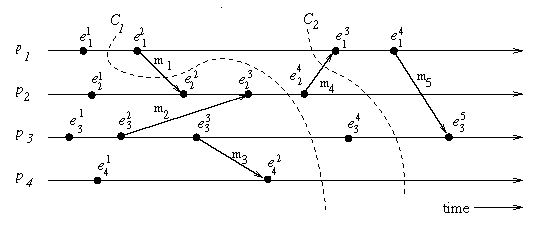
\includegraphics[width=1\linewidth]{48/example_cut.pdf}
    \caption{Příklad řezu v časoprostorovém diagramu. Řez $C_1$ je nekonzistentní, kvůli zprávě $m_1$. Řez $C_2$ je konzistentní a zpráva $m_4$ je zachycena ve stavu kanálu $Ch_{21}$.}
    \label{48_example_cut}
\end{figure}


\begin{figure}[H]
    \centering
    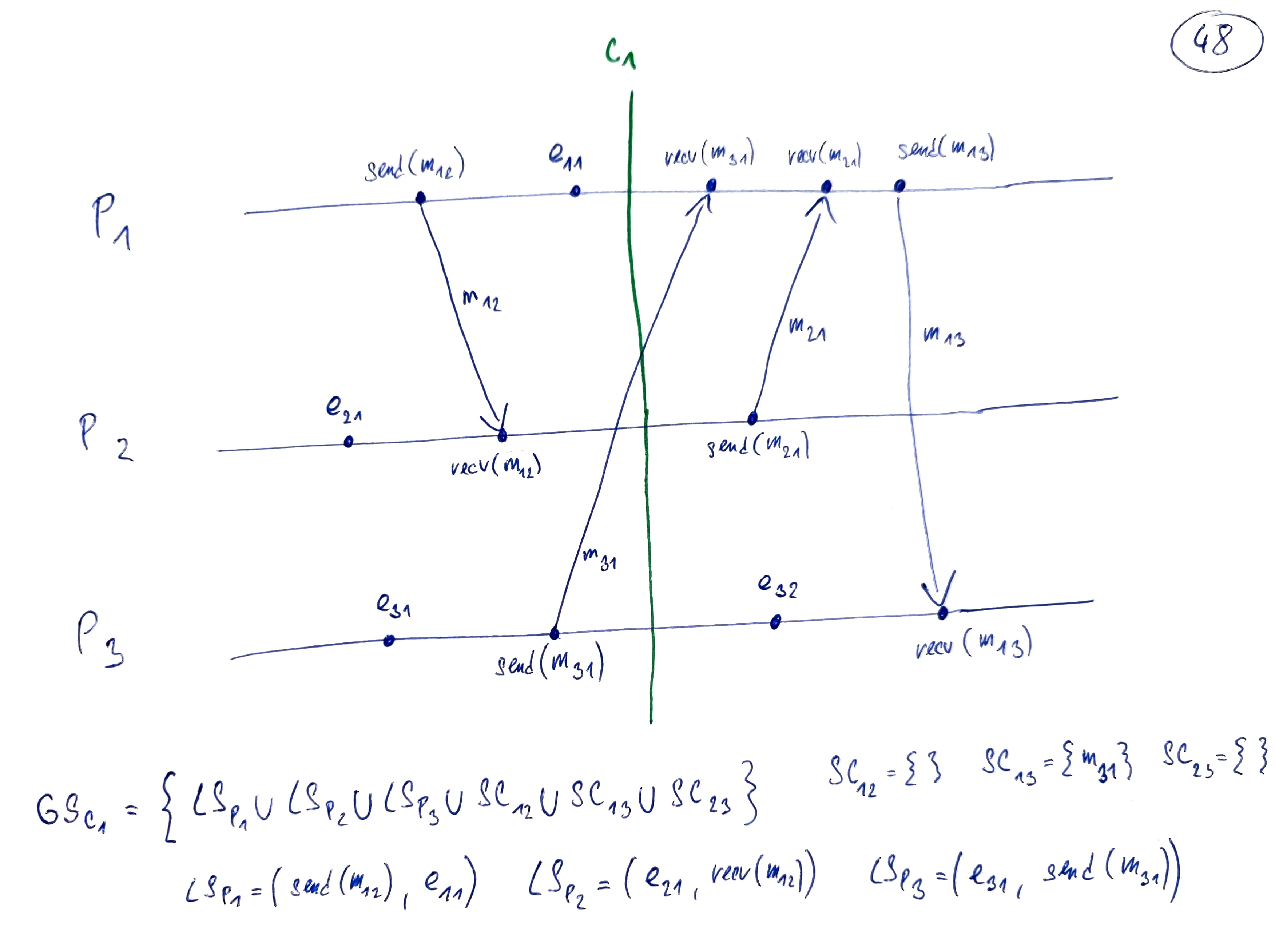
\includegraphics[width=1\linewidth]{48/example_consistent_state.pdf}
    \caption{Příklad konzistentního globální stavu formálně.}
    \label{48_example_consistent_state}
\end{figure}

\newpage

%%%%%%%%%%%%%%%%%%%%%%%%%%%%%%%%%%%%%%%%%%%%%%%%%%%%%%%%%%%%%%%%%%%%%%%%%%%%%%%%

\end{document}
